\documentclass[11pt, a4paper]{article}
\usepackage{fullpage}
\usepackage[utf8]{inputenc}
\usepackage[T1]{fontenc}
\usepackage{graphicx}
\usepackage{float}
\usepackage{amsmath}
\usepackage{amssymb}
\usepackage{listings}
\usepackage{hyperref}
\usepackage[french]{babel}
\usepackage{url}
\usepackage{comment}
\usepackage{xcolor}


\newcommand{\besoinVItem}[4]{
	\item #1
	\begin{description}
		\item[description :]
		#2
		\item[faisabilité: ]
		#3
		\item[cas d'utilisation :]
		#4
	\end{description}
}
\title{Apprentissage par renforcement multi-agents, De SlimeVolley à la RoboCup : Mémoire}
\author{Pélagie Alves\and Elias Debeyssac\and Alexis Hoffmann\and
Alexis Lhéritier\and Nicolas Majorel\and Sébastian Pagès}
\date{Mars/Avril 2021}

\begin{document}

	\maketitle

	\newpage

	\tableofcontents

	\newpage

	\section{Introduction}

	Le projet << Apprentissage par renforcement multi-agents : de SlimeVolley à la RoboCup >> nous est proposé par Ludovic Hofer qui est membre de l’équipe Rhoban, un groupe de recherche en robotique du LaBRI. Cette équipe travaille sur la robotique autonome et participe depuis presque 10 ans à la RoboCup, et notamment à la RoboCupSoccer\footnote{ On désignera désormais la RoboCupSoccer sous le nom de Robocup } qui est une compétition de football robotique. Notre client est spécialisé dans l'apprentissage par renforcement qui est une des méthodes utilisées pour entraîner les robots à jouer des matchs.\\
	Pour que les agents puissent développer des stratégies de jeu collectives, il faut réaliser l'apprentissage dans un contexte multi-agents. Les agents sont les robots qu'on entraîne et les stratégies définissent les comportement adoptés par les agents. Il s'agit de mettre en place une simulation de matchs de la RoboCup, dans laquelle des agents prennent des décisions de manière autonome tout en tenant compte des agissements, des modifications des éléments de la simulation\footnote{Les éléments pris en compte sont notamment la balle, les autres agents}. En fonction de l'impact positif ou négatif des décisions que les agents prennent lors du processus d'apprentissage, on leur attribue un score de récompense permettant de les encourager à répéter les comportements favorables à la victoire de l'équipe. On utilise une simulation pour entrainer les robots car cela permet d'accélérer l'entrainement et de moduler facilement les paramètres de l'entrainement.

	Notre objectif est donc d'implémenter une simulation de la RoboCup compatible avec l'apprentissage par renforcement multi-agents dans laquelle l'utilisateur peut activer et désactiver des options et règles afin de jouer sur la granularité de l'environnement. L'environnement est le contexte dans lequel les agents évoluent. \\
	Notre client devra pouvoir utiliser l'application pour entraîner des intelligences artificielles et évaluer l'efficacité des algorithmes d'apprentissage, les différents comportements des agents en fonction des environnements qu'il aura paramétrés et les stratégies qui en résultera.\\
	Nous ne devons pas fournir des IA performantes ou des algorithmes d'apprentissage mais une application qui devra pouvoir être utilisée afin d'entraîner des IA. Nous devons fournir une simulation sur laquelle il est possible de réaliser un apprentissage. Nous aurons besoin que notre application soit compatible avec les bibliothèques d'algorithmes d'apprentissage par renforcement classiques \footnote{comme tensorFlow ou stable-baseline} pour pouvoir les utiliser lors de l'apprentissage.

	Pour nous aider, notre client nous a fourni le projet SlimeVolleyGym de David Ha. Ce projet utilise la bibliothèque Gym pour créer un environnement d'apprentissage et entrainer des IA au jeu Slimevolley en se basant sur des algorithmes d'apprentissage de la bibliothèque stable-baseline. Slimevolley étant un jeu de balle en 2D tout comme la simulation de la Robocup que nous devons créer, nous nous appuierons sur SlimeVolleyGym pour le développement de la  simulation de la Robocup.\\
	Pour se familiariser avec la bibliothèque Gym et l’apprentissage par renforcement multi-agents, notre client nous propose dans un premier temps d’implémenter le mode deux contre deux ainsi que l'apprentissage de stratégie en deux contre deux dans le projet SlimeVolleyGym. Cette première partie servira de preuve de concept pour la simulation de la Robocup afin de montrer qu'il est possible d'entrainer des IA à jouer au jeu SlimeVolley en équipe, et que par conséquent il devrait être possible d'entrainer des IA à jouer des matchs de RoboCup.

	Tout d'abord nous allons présenter précisément le contexte dans lequel s'inscrit l'application. Puis nous décrirons les besoins qui ont guidés le développement. Nous présenterons ensuite l'architecture de l'application ainsi que les choix techniques que nous avons fait pour l'implémentation. Enfin nous fournirons une description et une analyse du fonctionnement de la Robocup. Nous terminerons par des exemples de test de SlimeVolley Multi-agents et de la Robocup.


	\section{Contexte}


	La Robocup étant un jeu d'équipe, il est nécessaire pour avoir les résultats les plus intéressants, d'entrainer les agents dans un contexte multi-agents \footnote{Plusieurs agents autonomes dans la même équipe}. Nous allons donc définir différents concepts qui permettent d'appréhender l'apprentissage par renforcement multi-agents sur lesquels nous nous sommes appuyés pour implémenter la simulation.\\
	Dans cette partie décrivant le contexte nous allons premièrement préciser l'intérêt de notre projet, ensuite nous présenterons l'apprentissage par renforcement (quelques généralités), puis nous allons entrer un peu plus dans les détails avec les processus décisionnels de Markov, et enfin nous parlerons de la bibliothèque Gym et du projet SlimeVolleyGym qui en est un exemple d'utilisation.\\


	Le but est que notre client puisse développer différentes stratégies/politiques d'IA en fonction de l'environnement d'entraînement. En effet, modifier l'environnement a une influence sur l'apprentissage. L'intérêt est d'observer l'impact d'une option dans l'apprentissage. Pour tester les différentes stratégies et environnement, on fait s'affronter 2 politiques différentes dans divers environnements et on analyse les résultats. Ainsi on verra la corrélation entre environnement et succès d'une stratégie.
	La complexité de l'environnement a aussi un impact sur la durée de l'apprentissage : plus la granularité de l'environnement est forte plus il se rapproche de la réalité mais plus l'apprentissage est long.  C'est pourquoi il est parfois intéressant de commencer un apprentissage sur un environnement simple et de l'affiner vers un environnement plus complexe. Avec python, on peut réaliser des tests pour évaluer le temps d'apprentissage en fonction des algorithmes, de l'environnement d'entraînement et de la politique contre laquelle l'IA s'entraine, ce qui augmente encore l'intérêt de Gym pour réaliser ce projet.

	De plus la simulation devra être implémentée de manière à pouvoir rajouter des règles pour s'adapter à la véritable Robocup qui changent tous les ans pour challenger la performance des robots.\\

	Nous allons maintenant présenter les concepts clé derrière notre projet e commençant par l'apprentissage par renforcement.

	\subsection{Apprentissage par renforcement et multi-agents}
	L'apprentissage par renforcement est une méthode d'apprentissage qui consiste a récompenser ou punir les agents (entités autonomes de la simulation) en fonction des actions qu'ils accomplissent. L'idée est de laisser l'agent apprendre de ses erreurs. Par exemple, si on pénalise l'agent pour  un certain comportement, il peut renoncer à celui-ci, si on le récompense cela va au contraire l'encourager à le reproduire.

	Dans l'apprentissage par renforcement,les éléments principaux sont  l'agent et l'environnement. L'environnement est le modèle dans lequel évolue les agents à un instant donné, il prend également en compte l'observation de l'agent c'est-à-dire ce qu'il perçoit du modèle. La récompense que l'agent reçoit fait également partie de l'environnement. Ce nombre est un indicateur de l'évaluation du comportement de l'agent pour un environnement donné. L'objectif de l'agent est de maximiser son score de récompense c'est pour cela qu'il répète des comportements jugés positifs par l'environnement et élabore une stratégie adaptée à celui-ci.\\

	Le multi-agent est un système composé de multiple agents qui sont dans le même environnement et interagissent. Pour qu'un environnement soit caractérisé comme étant multi-agent il faut respecter plusieurs règles : les agents doivent être autonomes et prendre leurs décisions seul (décentralisé), les agents doivent avoir une vision locale de l'environnement et les agents doivent être autonomes c'est-à-dire qu'ils n'ont pas besoin de l'utilisateur pour agir.

	\subsection{Processus décisionnel de Markov}

	On illustre souvent les concepts fondamentaux de l'apprentissage par renforcement avec le processus de décision markovien :
	$$\left\langle \mathbf{S}, \mathbf{A}, \mathbf{T}, R, P\right\rangle$$

	\noindent$\mathbf{S} :$ est l’espace d’états dans lequel évolue le processus,  c'est un ensemble dénombrable ou continu \\
	$\mathbf{A} :$ est l’espace des actions qui contrôlent la dynamique de l’état, c'est un ensemble dénombrable ou continu  \\
	$\mathbf{T} :$ est l’espace des temps, ou axe temporel\\
	$R : \mathbf{S} \times \mathbf{A} \times \mathbf{S} \rightarrow \mathbb{R} $, la fonction de récompense, avec $r_t = \mathbf{R}\left(s_t, a_t, s_{t+1}\right)$  \\
	$P :$ est la fonction de probabilité de transition entre les états $s_t$ et $s_{t+1}$ en exécutant l'action a : $\mathcal{P} \left(s_{t+1}|s_t,a\right)$

	\vspace{0.5cm}

	\noindent Tous les états ont la propriété «Markov», faisant référence au fait que l'avenir ne dépend que de l'état actuel.

	\noindent \textbf{S} : L'état est la description de l'environnement à un instant t perçu par un agent. \\
	Dans SlimeVolley l'état comprend différents éléments : la position de la balle et des agents, la vitesse de la balle et des agents. L'espace d'observation peut être partiel ou complet. Dans un espace d'observation complet, les agents perçoivent tous les éléments du jeu, alors que dans un espace d'observation partiel certains éléments sont masqués. \\
	Voici l'espace d'état dans SlimeVolley :

	$$
	\begin{bmatrix}
		x\_agent & y\_agent & \dot{x} \_agent & \dot{y}\_agent \\
		x\_ball & y\_ball & \dot{x}\_ball & \dot{y}\_ball \\
		x\_opponent & y\_opponent & \dot{x}\_opponent & \dot{y}\_opponent \\
	\end{bmatrix}
	\label{tab_state}
	\quad
	$$


	\noindent \textbf{A} : L'espace d'action représente toutes les possibilités d'actions pour l'agent dans le modèle. Dans le cadre de SlimeVolley il s'agit des déplacements des agents : avancer, reculer, sauter.
	Il peut arriver que ces déplacements soient contraints par exemple l'agent ne doit pas sortir de sa moitié de terrain. Dans ce cas, si on accède à un déplacement non autorisé, alors il n'est pas appliqué.\\
	Voici l'espace d'action dans SlimeVolley :
	$$
	\begin{bmatrix}
		forward & backward & jump
	\end{bmatrix}
	$$

	\noindent \textbf{R} : La récompense est attribuée à l'agent en fonction de ses actions. Pour SlimeVolley, si l'agent marque un point alors il reçoit +1 en récompense en revanche s'il rate la balle et la laisse tomber il reçoit -1.

	\begin{figure}[H]
		\centering
		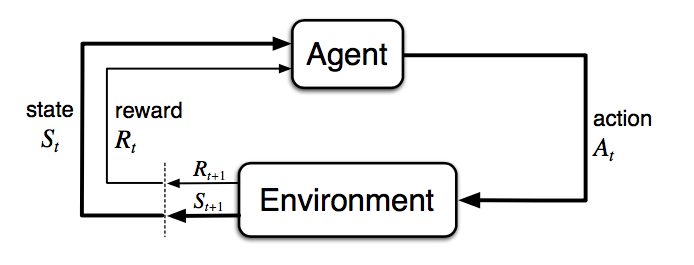
\includegraphics[scale=0.5]{images/agent_environment_MDP.png}
		\caption {Schéma du processus décisionnel de Markov \cite{schemamarkov}}
	\end{figure}


	Maintenant que nous avons défini les concepts de base de l'apprentissage, nous allons introduire la bibliothèque Gym et plus particulièrement l'environnement Gym qui s'appuie sur les processus décisionnels de Markov.

	\subsection{Bibliothèque Gym et environnement Gym}

	Gym est une bibliothèque python permettant de développer et comparer des algorithmes d'apprentissage par renforcement. Elle a été conçue par OpenAI pour palier au manque d'environnements variés dans le domaine du RL\footnote{Reinforcement Learning} et à leur difficulté d'utilisation. En effet, Gym permet de créer des environnements personnalisable à l'aide d'une interface partagée et a pour ambition de standardiser les environnements pour faciliter la comparaison et la réutilisation de résultats provenant des publications scientifiques sur l'apprentissage par renforcement. Elle est aussi compatible avec de nombreuses/toutes bibliothèques d'algorithmes de RL comme stable-baseline ou encore tensorFlow et a pour objectif d'être la référence dans le domaine du RL\cite{openaigym}.

	\vspace{0.5cm}

	Un environnement Gym : \textbf{env} est composé d'un espace d'action : \textbf{A} \textit{(action\_space)}, qui contient les actions possibles pour les agents, d'un espace d'observation : \textbf{S} \textit{(observation\_space)}, qui représente la vision qu'ont les agents de l'environnement et d'une récompense \textbf{R} \textit{(reward)} pour l'apprentissage de l'agent, c'est une valeur flottante. On doit choisir combien de pas de temps l'environnement va exécuter.

	\vspace{0.5cm}

	Dans Gym, il existe plusieurs types d'\underline{espace d'actions} comme \textit{Discrete} qui attribut à une action un numéro entre 0 et N-1\footnote{ici N est le nombre d'actions disponibles dans l'environnement}. Il y a aussi un espace \textit{MultiBinary} qui défini un espace binaire de dimension N.
	Dans la version de David Ha il y avait ces 2 types d'espace d'actions mais dans notre version SlimeMultiAgent on a choisi d'utiliser uniquement l'espace discret.

	L'\underline{espace d'observation} est de type \textit{Box} qui est un tenseur à N dimensions qui prend en compte des coordonnées d'un certains type qui se situent entre 2 valeurs.
	Dans la version de base de SlimeVolley il y a 2 types d'espace d'observation: un par état (\textbf{S}) et un par pixels. Le type influencera l'apprentissage de l'agent.

	\begin{itemize}
		\item Avec un mode par état l'agent reçoit les informations décrites dans \ref{tab_state}, ces données sont du type float32. On a un vecteur de taille 12 avec des valeurs qui se situent entre le maximum et le négatif du maximum des valeurs du vecteur.
		Voila ce que l'on obtient lorsque l'on affiche l'espace d'observation par état :
		\begin{figure}[H]
			\centering
			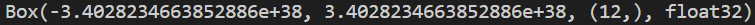
\includegraphics[scale=0.5]{images/obs_spaceBox.PNG}
			\caption {Espace d'observation par état dans slimevolleygym}
		\end{figure}

		\item Avec un mode d'observation par pixel on a une image de 84*168 pixel en RGB, le type est donc uint8.
		\begin{figure}[H]
			\centering
			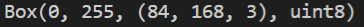
\includegraphics[scale=0.5]{images/obs_spaceBoxPixel.PNG}
			\caption {Espace d'observation par pixel dans slimevolleygym}
		\end{figure}
		Dans le mode pixel, les informations sont moins précises car elles doivent être extraites à partir d'images de l'environnement. L'apprentissage peu être plus lent car il a y a plus d'informations à traiter.
	\end{itemize}

	C'est pourquoi dans notre simulation nous utiliserons uniquement le mode d'observation par état.

	\vspace{0.5cm}

	L'\textbf{env} de Gym contient les fonctions suivantes : \cite{openaigymenv}
	\begin{itemize}
		\item  \textbf{step} qui exécute un pas de temps de l'environnement et retourne une récompense, l'observation de l'agent, un booléen \textit{done} pour déterminer si la simulation est terminée et \textit{info} qui aide à l'apprentissage et au debuggage.
		\item \textbf{reset} qui réinitialise l'environnement à son état original et à son espace d'action d'origine.
		\item \textbf{render} qui permet de gérer l'affichage de l'environnement et la sortie d'un environnement en fonction de l'option choisi.
		\item \textbf{close} qui détruit l'environnement.
		\item \textbf{seed} qui permet de générer un nombre pseudo aléatoire pour l'environnement.
	\end{itemize}

	Pour illustrer le fonctionnement de Gym nous allons vous présenter le projet de RL SlimeVolleyGym qui servira de preuve de concept pour la RobocupGym.

	\subsection{SlimeVolleyGym}

	SlimeVolleyBall est un jeu des années 90 dans lequel deux slimes disputent un match de volley. Chaque slime a un nombre de vie et dès que la balle touche le sol dans sa moitié de terrain, il perd une vie. Quand le compteur de vie d'un des slime tombe à 0, la partie se termine. On peut jouer à slimevolley en local sur le même clavier ou contre une IA.\\
	Il y a trois actions possibles : se déplacer vers la droite, vers la gauche et sauter.

	\vspace{0.5cm}

	SlimeVolleyGym \cite{slimevolleygym} est un projet d'apprentissage par renforcement développé par David Ha, c'est une adaptation en python de son projet javascript \cite{ha2015slimevolley} de 2015.
	À l'aide de la bibliothèque Gym, il a reproduit l'environnement du jeu SlimeVolleyBall afin d'y réaliser des expériences d'apprentissage par renforcement.

	Voila à quoi ressemble slimeVolley, nous détaillerons les différents environnements dans la partie \ref{tab_env}.
	\begin{figure}[H]
		\centering
		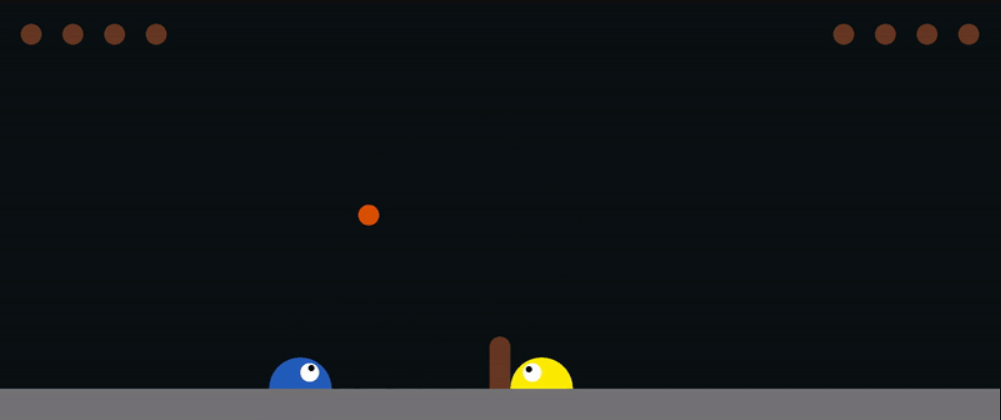
\includegraphics[scale=0.5]{images/slimeVolley.PNG}
		\caption {Image de l'environnement slimeVolley-v0  \cite{slimevolleygym}}
	\end{figure}

	Le but de ce projet est de pouvoir entraîner des IA avec différents algorithmes d'apprentissage et contre différentes politiques d'adversaire, pour ensuite évaluer l'apprentissage. On se base sur le score de l'agent entraîné contre la baselinePolicy qui est l'IA que David Ha avait entrainé dans son précédent projet. Les algorithmes testés sont principalement PPO, CMA-ES \footnote{Proximal Policy Optimization et Covariance Matrix Adaptation Evolution Strategy sont des algorithmes de RL, nous n'expliquerons pas leur fonctionnement car nous devons juste pouvoir les utiliser}. On récupère les résultats des entraînements et les scores grâce à des scripts python. \\
	Dans le code nous avons plusieurs script d'apprentissage déjà entrainé qui on servit à faire des évaluation d'apprentissage en fonction de différents environnements. Malheureusement nous ne pouvons pas utiliser ces scripts\footnote{On peut retrouver tous les scripts sur le git de David Ha dans le dossier trainning\_scripts} car ils datent de 2015 et sont obsolètes.\\

	Une autre fonctionnalité de SlimeVolleyGym est de pouvoir jouer à SlimeVolleyBall contre un ami en local ou contre baselinePolicy. Les scripts "jouables" sont les fichiers test\_state.py, test\_pixel.py et test\_atari.py. Il y a plusieurs fichiers pour plusieurs environnements, nous détaillerons les différents environnement\ref{tab_env} qui seront décrit plus bas. D'ailleurs il est très difficile de marquer un point contre baselinePolicy.

	Pour résumer le fonctionnement de slimeVolleyGym voici un diagramme de cas d'utilisation.
	\begin{figure}[H]
		\centering
		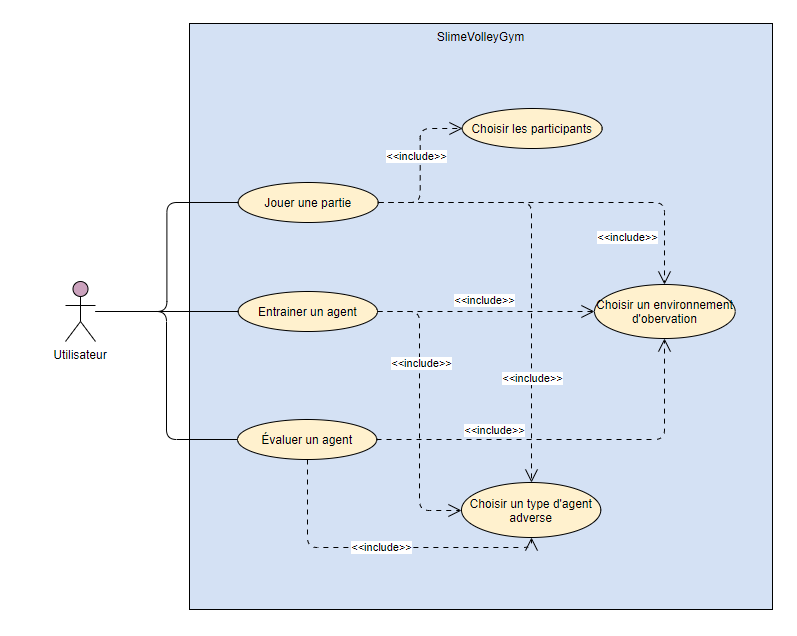
\includegraphics[scale=0.6]{images/cas_utilisation.PNG}
		\caption {Diagramme de cas d'utilisation de SlimeVolleyGym}
	\end{figure}

	Dans ce projet il y a plusieurs environnements comme l'illustre le tableau ci-dessous, le mode d'observation est soit par pixels, soit par états. D'autres environnement on est mode de jeu différent : au lieu d'avoir 5 vie par agent et de perdreune vie à chaque fois que la balle tombe, on peut jouer dans un environnement où les agents coopèrent pour but de ne pas faire tomber la balle. Cet environnement utilise le multi-agent car les agents partagent la récompense puisqu'ils sont considérés comme allié.
	Dans SlimeVolleyGym, le mode d'observation par état prend en compte les coordonnées, la vitesse de l'agent, son adversaire et la balle, il s'agit donc d'un vecteur à 12 dimensions. Dans le mode d'observation par pixels, on a des images de 84*168 pixels. Il y a aussi des différences dans la manière de représenter l'espace d'actions mais cela ne nous intéresse pas. Dans la pratique on utilise l'environnement slimeVolley-v0 qui correspond au mode d'observation par états, on appellera ce mode state et slimeVolleyNoFrameskip-v0 qui représente le mode d'observation par pixels que l'on nommera pixel.

	\begin{figure}[H]
		\centering
		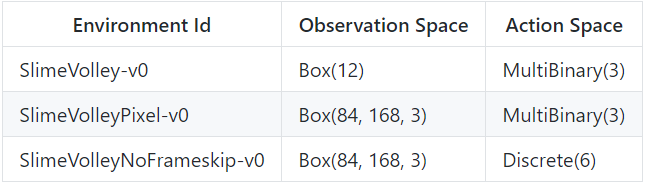
\includegraphics[scale=0.8]{images/environnementsS.PNG}
		\caption {Liste des différents environnements de SlimeVolleyGym et leurs caractéristiques \cite{slimevolleygym}}
		\label{tab_env}
	\end{figure}
	\begin{figure}[H]
		\centering
		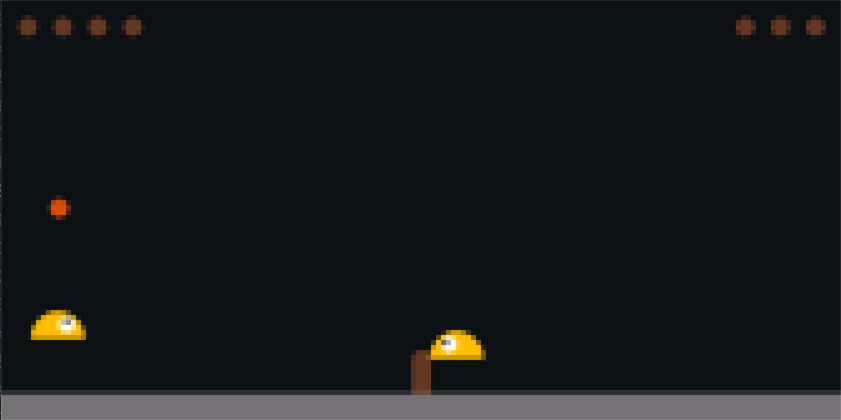
\includegraphics[scale=0.6]{images/slimeVolleyPixel.PNG}
		\caption {Image de l'environnement slimeVolleyNoFrameskip-v0 \cite{slimevolleygym}}
	\end{figure}


	Le jeu et l'environnement Gym (slimeVolleyEnv) sont implémentés dans le fichier slimevolley.py. La classe \textbf{SlimeVolleyEnv} est une implémentation de l'interface Env d'un environnement Gym. \\
	Dans slimeVolleyGym, il est possible d'avoir différents mode de jeu comme survival où l'agent reçoit une récompense en fonction du temps qu'il a tenu avant de faire tomber la balle. On peut aussi changer le mode d'observation par défaut(state) par une observation par pixel.\\
	Pour gérer les modes/environnements, il y a plusieurs classes qui contiennent des booléens et modifient les variables locales de la classe \textbf{SlimeVolleyEnv} qui par défaut correspond à l'environnement \textit{slimeVolley-v0}. La classe \textbf{SlimeVolleyAtariEnv} correspond à l'environnement \textit{slimeVolleyNoFrameskip-v0}, la classe \textbf{SlimeVolleyPixelEnv} correspond à \textit{slimeVolleyPixel-v0}. Même principe avec les classes \textbf{SurvivalRewardEnv} et \textbf{SlimeVolleySurvivalAtariEnv}.\\
	Une fois l'environnement créé, il faut le sauvegarder pour pouvoir l'utiliser, les noms de sauvegarde sont en gras, pour générer l'environnement state on fait \textbf{ env = gym.make("SlimeVolley-v0")}. Les options de chaque environnement sont développées dans le tableau figure \ref{tab_env} .\\
	Voir ci-dessous le diagramme de classe.

	\begin{figure}[H]
		\centering
		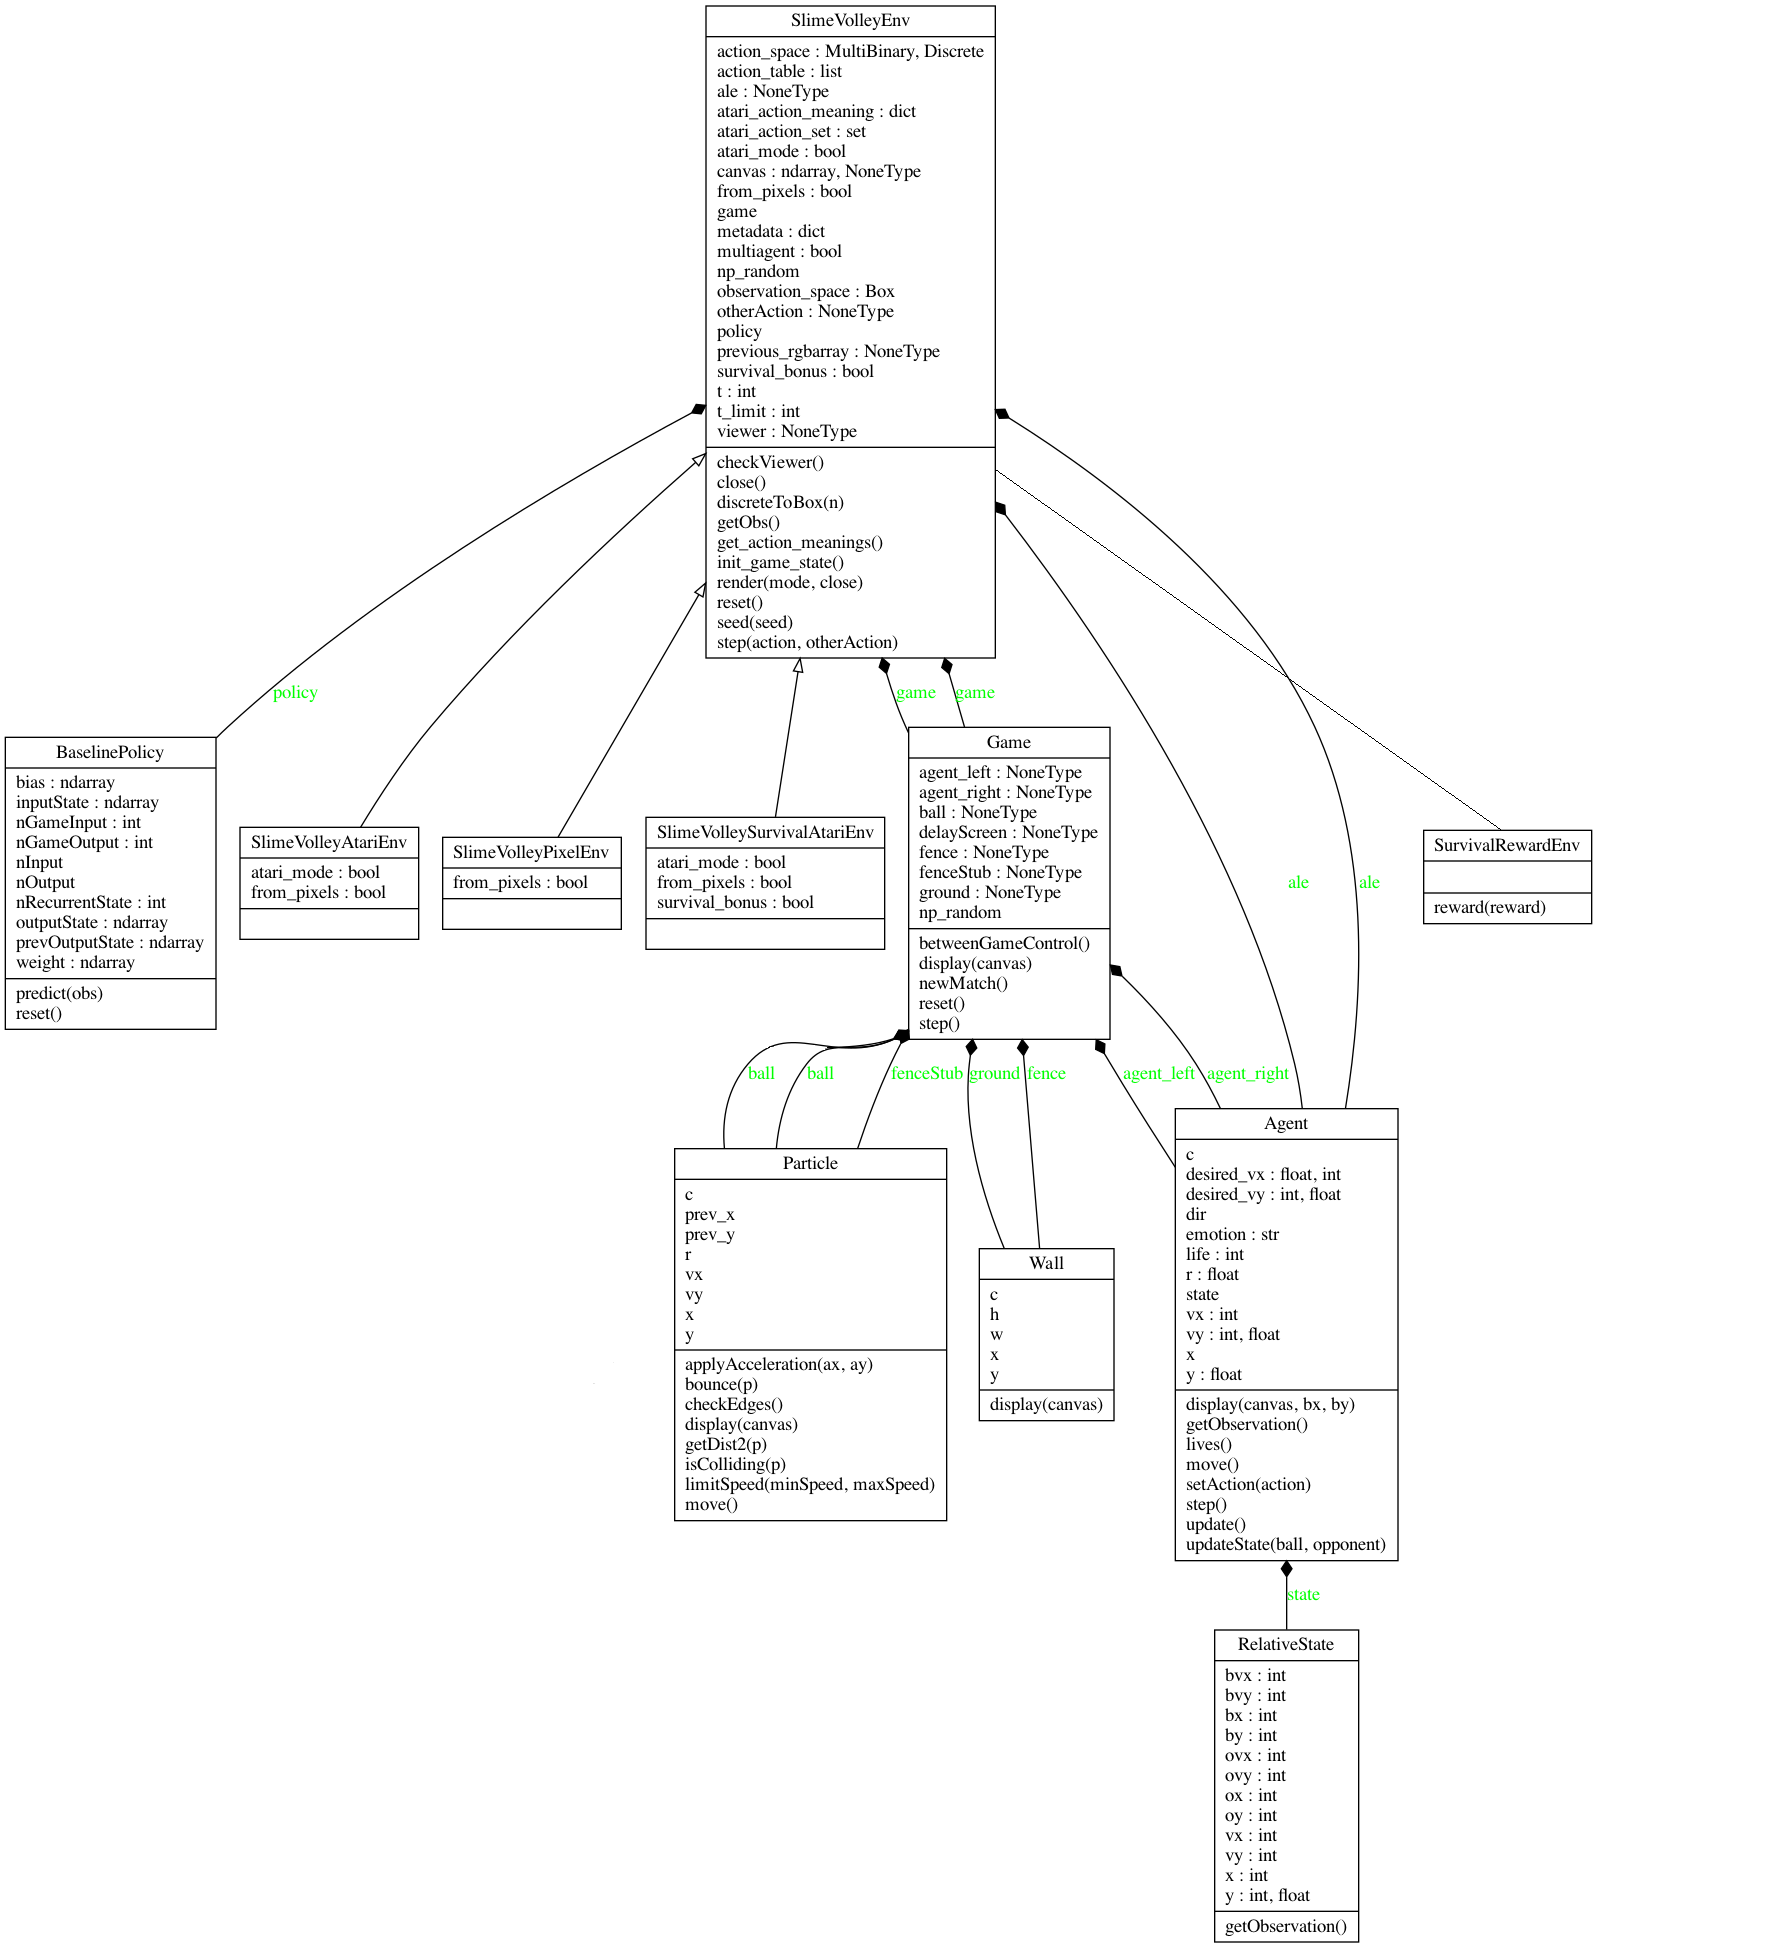
\includegraphics[scale=0.5]{images/classes.png}
		\caption {Diagramme de classes de SlimeVolleyGym}
	\end{figure}

	Pour créer un environnent slimeVolleyBall il faut d'abord définir les éléments principaux, leurs interactions et leur affichage:
	\begin{itemize}
		\item La classe \textbf{Particule} définit la balle et ses différentes actions (affichage, déplacement, test de collision, rebond et vitesse max). Cette classe prend en entrée la position x et y de la balle, ses vecteurs de vitesse vx et vy, son rayon r et sa couleur c.
		\item La classe \textbf{Agent} définit un agent, ses actions (sauter, se déplacer dans le terrain). L'agent prend en entrée sa position x et y, une couleur c et sa position sur le terrain (côté droit(1) ou côté gauche(-1)).
		\item La classe \textbf{RelativeState} qui sauvegarde l'observation par état précédent et actuel d'un agent. La classe est utilisée par la classe Agent pour garder une trace de l'état du jeu après chaque action. Les éléments sauvegardés dans l'état sont, la position et le vecteur vitesse de l'agent lui-même, de son adversaire et de la balle.
		\item La classe \textbf{Wall} permet de définir le mur séparant les deux joueurs (filet) et le sol sur lequel les joueurs se déplacent. Les valeurs d'entrées nécessaires sont la position en x et y, sa longueur w, sa hauteur h et sa couleur c.
	\end{itemize}
	\begin{figure}[H]
		\centering
		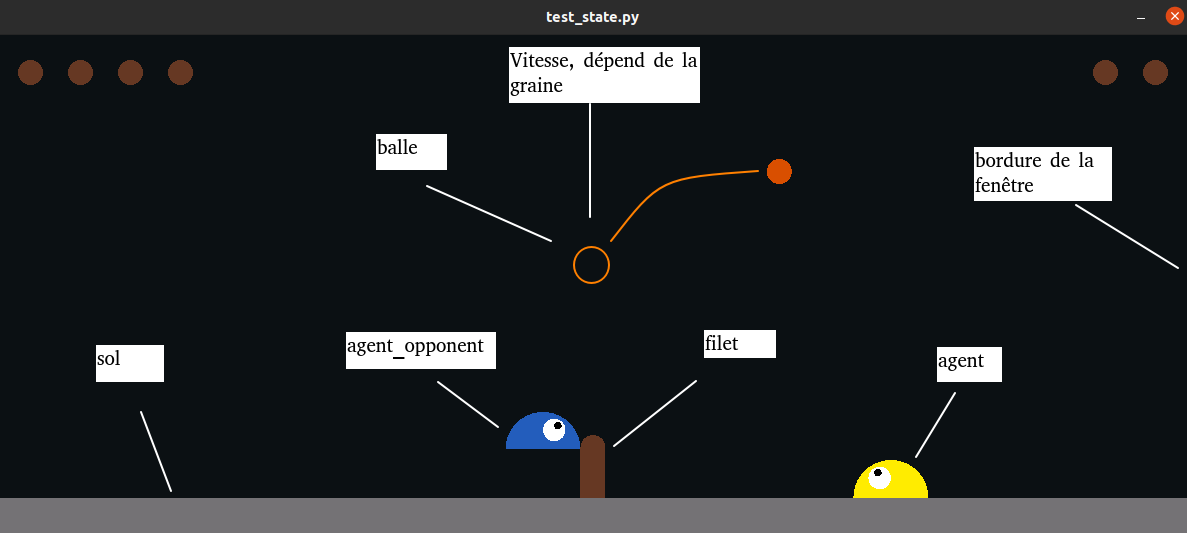
\includegraphics[scale=0.4]{images/schema.png}
		\caption {Les différents éléments de SlimeVolleyGym \cite{slimevolleygym}}
	\end{figure}

	Tous ces éléments sont ensuite gérés par la classe \textbf{Game} qui est utilisé dans SlimeVollyEnv. Game gère l'initialisation de la partie, affiche les éléments à l'écran, lance/réinitialise/arrête un match, gère le nombre de vies restantes par agent, le gagnant et le perdant. Elle contient également la boucle de jeu qui à chaque étape, s'occupe de déplacer les agents et de la balle, vérifie la collision entre un agent et la balle et actualise l'observation de chaque Agent. Elle prend en entrée un nombre aléatoire qui sera la graine de jeu de la partie.

	\vspace{0.5cm}

	La classe \textbf{BaselinePolicy} reprend les paramètres du réseau de neurones entrainé du précédent projet de David Ha \cite{ha2015slimevolley}. Elle sert de référence pour évaluer l'apprentissage et d'adversaire pour l'entraînement.

	\vspace{0.5cm}

	Pour rentrer plus en détail dans le fonctionnement de SlimeVolleyGym on a fait un diagramme de séquence lors de l'exécution du script \textit{test\_state.py}.

	\begin{figure}[H]
		\centering
		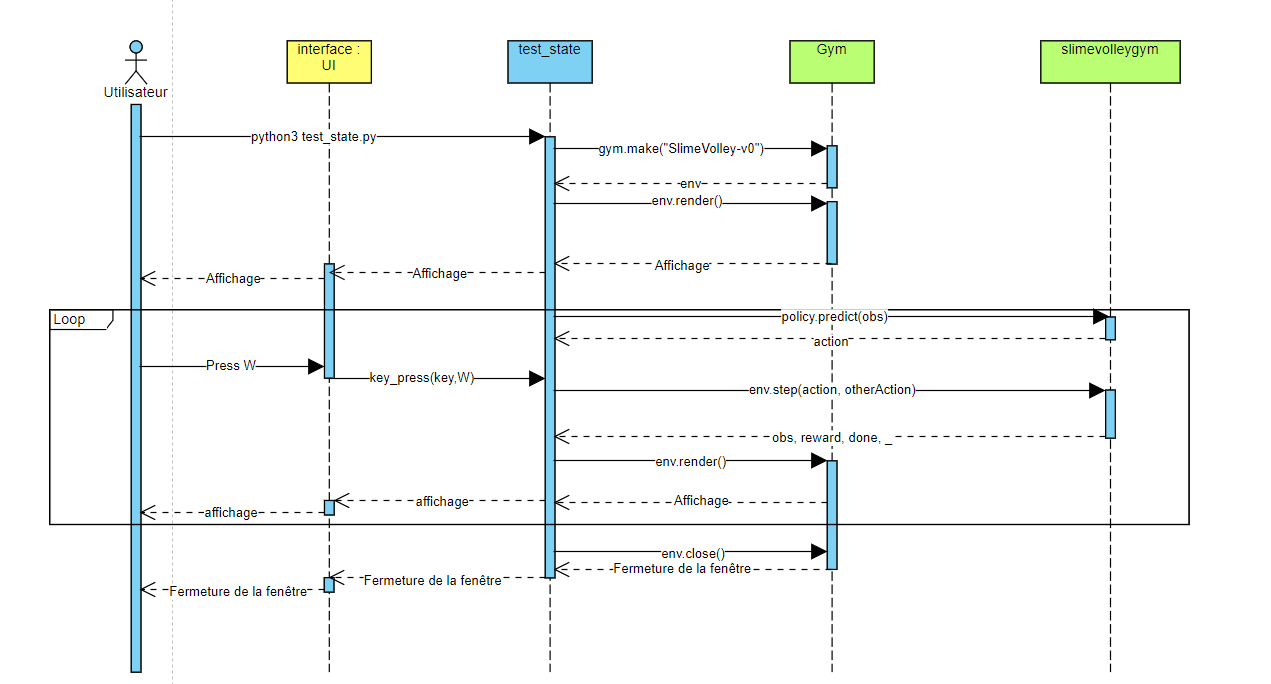
\includegraphics[scale=0.5]{images/diagramme_sequence.PNG}
		\caption {Diagramme de séquence lors de l’exécution du fichier test\_state.py en mode Humain contre Machine}
	\end{figure}

	Pour lancer des entrainements, des évaluations ou jouer, il faut utiliser des scripts. \\
	Lorsque l'utilisateur lance le script test\_state, l'environnement gym est généré avec gym.make() puis, la fonction de \textbf{render} de l'environnement génère l'affichage du jeu. On entre dans la boucle de jeu : l'IA qui choisit ses actions avec policy.predict(obs) en fonction de ce qu'elle perçoit, c'est-à-dire, l'espace d'observation renvoyé par \textbf{step} tandis que l'utilisateur appuie sur une touche du clavier qui est reliée à une action. Dans les deux cas, l'action est transmise à env.step() qui l'exécute et met à jour l'affichage et l'espace d'observation des agents. \textbf{step} renvoie le nouvel espace d'observation, la récompense et si la partie est terminée. La récompense est donnée par rapport à l'agent de droite, il reçoit 0 s'il ne se passe rien, 1 s'il marque et -1 s'il prend un point. Si l'agent de gauche marque, il recevra -1 et s'il perd 1. Dans ce script, l'action est un vecteur binaire de dimension 3.

	\vspace{0.5cm}

	Pour obtenir plus d'informations concernant le projet SlimeVolleyGym, vous pouvez consulter le git de hardmaru \cite{slimevolleygym}.

	\vspace{0.5cm}

	\section{Analyse des besoins}

	\subsection{Organisation}

	Pour l'extension de SlimeVolley nous avons le code de SlimeVolleyGym en enlevant les parties inutiles pour faire un environnement multi-agent de 2vs2. Cet environnement est de type state.
	\vspace{0.5cm}
	Pour la Robocup, nous devions créer une simulation capable de fournir divers environnements d'entrainement et d'évaluation.
	Nous nous sommes inspirés de l'architecture et des classes de slimeVolleyGym mais nous avons refactorisé le code. Là aussi nous avons implémenté des environnements seulement avec le mode d'observation state.
	Idéalement nous devions rajouter le plus d'options possibles pour qu'elle se rapproche au maximum des conditions de la vrai Robobocup.
	\vspace{1cm}

	On décrira la liste des besoins fonctionnels et non-fonctionnels relatifs à l'implémentation du multi-agents dans Slime Volley Gym et la simulation de la RoboCup ci-dessous. On donnera des niveaux de priorité à ces besoins selon la classification suivante :

	\begin{itemize}
		\item \textit{Mandatory} : les besoins obligatoires et nécessaires au bon fonctionnement de l'application.
		\item \textit{Important} : les besoins qu'il serait important d'implémenter afin de rendre l'application intéressante.
		\item \textit{Optional} : les besoins optionnels qui permettraient d'enrichir l'application et de la rendre plus paramétrable.
	\end{itemize}

	Les besoins réalisés seront en \textcolor{red}{rouge}, les besoins partiellement réalisés seront en \textcolor{violet}{violet} et les besoins non réalisés seront en \textcolor{olive}{vert kaki}.

	\subsection{Besoins pour l'environnement 2vs2 multi-agents de SlimeVolley nommé slimultiagent}
	Le premier besoin est de définir un environnement avec quatre agents, deux par équipe, dans lequel les agents doivent prendre des décisions seul mais en étant influencé par leur environnement. Des agents qui coopèrent auront la même récompense. Cet environnement s'appelle slimultiagent.\\
	Ensuite il faut que slimultiagent soit fonctionnel, c'est-à-dire que l'on puisse entrainer un agent avec. \\
	Le dernier besoin est pouvoir évaluer notre apprentissage en le faisant se confronter à une autre IA. Dans notre cas on évaluera  l'apprentissage en le confrontant à une IA qui joue de manière aléatoire.\\
	\subsubsection{Ajouter des agents à SlimeVolleyGym pour avoir du 2 vs 2 et créer l'enviornnement slimultiagent}
	\begin{enumerate}
		\besoinVItem{\textcolor{red}{Faire une équipe de 2 agents}    \textit{Mandatory}}
		{
			Avec le projet SlimeVolleyGym de Hardmaru on peut entrainer un Agent à slime-volley en 1 contre 1. L'agent entrainé sera donc plus fort que l'adversaire contre qui il s'est entrainé puisqu'il a pu développer des stratégies contre cet agent. On est dans un contexte d'apprentissage par renforcement single-agent. La première étape pour passer au multi-agents est de rajouter un joueur de chaque coté du filet pour créer un environnement gym où deux agents s'affrontent à slime-volley. Le but est d'avoir un environnement avec 2 équipes de 2 agents qui jouent à slime-volley pour pouvoir ensuite les entrainer et leur apprendre des stratégie à slime-volley en 2 contre 2. \\
			On devra pouvoir affecter une politique (manière de jouer, stratégie) comme un algorithme (random ou politique issue d'un entrainement préalable) à l'équipe contre laquelle on entraine l'agent. De plus pour faciliter la visibilité des joueurs et savoir quel agent on entraine (à l'affichage) on peut leur donner un numéro ou une couleur spécifique.
		}
		{
			On peut créer une classe \textbf{Team} qui aura un dictionnaire qui contiendra 2 agents. Pour créer les agents, la classe \textbf{Game}  appellera donc la classe \textbf{Team}.
		}
		{
			A chaque fois qu'on lance une session d'entrainement ou qu'on lance un match de test ce besoin va être utilisé puisque les équipes vont dorénavant être instanciées lorsqu'il y aura plusieurs joueurs par équipe dans SlimeVolleyGym.
		}




		\besoinVItem{\textcolor{red}{Adapter les fonctions/fonctionnalités d'un agent à une équipe} \textit{Mandatory}}
		{
			Dans SlimeVolleyGym, il y a l'objet Agent qui permet de gérer les joueurs. Pour passer du 1 contre 1 au 2 contre 2 à slimevolley, nous avons créé un objet Team qui peut contenir plusieurs Agent. Cette classe doit être compatible avec les fonctionnalités de l'environnement gym déjà existant afin que l'apprentissage soit toujours possible après son implémentation. Nous avons  du adapter les fonctionnalités précédemment gérées par la classe \textbf{Agent} à la classe \textbf{Team}. Nous avons donc encapsulé l'Agent dans la Team.
		}
		{
			Pour que le jeu continue de fonctionner il faut redéfinir les fonctions  présentes auparavant dans la classe Agent. Notamment les fonctions qui permettaient de gérer les actions en jeu, de mettre à jour l'état des agents, la fonction d'affichage et l'attribut permettant de récupérer le score.
		Ce sont les fonctions setactions(), update(), display() et l'attribut lives.
		}
		{
			Comme ce besoin découle du précédent, on a le même cas d'utilisation.
		}



		\besoinVItem{\textcolor{red}{Gérer les collisions entre agents d'une même équipe} \textit{Important}}
		{
			Nous avons voulu géré la collision entre agent d'une même équipe dans notre extension de SlimeVolleyGym. En effet ce besoin sera très important pour la Robocup c'est pourquoi nous avons décidé de l'implémenter à ce stade du
			développement. Nous avons donc fait en sorte que les hitbox des agents d'une même équipe ne puissent pas se superposer. En d'autres termes qu'ils se bloquent s'ils se touchent et qu'ils ne puissent pas se traverser.
		}
		{
			Pour réaliser ce besoin on peut créer des fonctions calculant la distance entre agents, ainsi qu'une fonction de vérification de collision. Ce principe de collision est déjà présent dans SlimeVolleyGym pour la collision entre un agent et la balle, il sera donc aisé de l'adapter pour une collision agent/agent. Il existe des algorithmes très complexes pour gérer la collision (surtout lorsque le nombre d'objet dans la simulation est très grand) mais ici un alorithme "naïf" nous suffit car on doit la vérifier qu'entre 2 objets.
		On pourrait utiliser les fonctions getDistance() et isColliding() de SlimeVolleyGym et les redéfinir dans la classe \textbf{Team}.
		Notre application devant être configurable, il faudrait que la collision le soit et qu'on puisse la désactiver.
		}
		{
			On pourrait faire en sorte que la collision soit un comportement négatif (reward négatif aux agents lorsqu'ils entrent en collision). Cela pourrait être intéressant de voir les agents apprendre une stratégie où ils limitent le plus possible d'entrer en collision. On pourrait comparer cette politique à une autre où les agents auraient été entrainés dans un environnement sans collisions et les faire s'affronter par exemple.
		}

	\end{enumerate}

	\subsubsection{Pouvoir entrainer et évaluer un agent dans l'environnement slimultiagent}
	\begin{enumerate}

		\besoinVItem{\textcolor{red}{Lancer une session d'entrainement }\textit{Mandatory}}
		{
			Maintenant que nous possèdons nos équipes de 2 slimes prêtes à jouer à slime-volley, il faut pouvoir réaliser l'apprentissage. L'implémentation des agents et de l'environnement devraient comporter toutes les caractéristiques nécessaires à l'apprentissage(détaillées dans les besoins précédent sur l'environnement gym). Il ne reste plus qu'à créer un exécutable permettant de faire jouer automatiquement les agents un grand nombre de parties contre une IA afin qu'ils apprennent de leurs erreurs, progressent et finissent par être meilleurs que cette IA. Dans notre extension on se concentrera sur l'apprentissage par renforcement d'un seul agent dans l'équipe.\label{session}
		}
		{
			Dans SlimeVolleyGym, il y a plusieurs scripts python d'apprentissage comme $train\_ppo.py$, $train\_ga\_selfplay.py$ \footnote{GA pour algorithme génétique qui s'inspire de la théorie de l'évolution de Darwin et de la sélection naturelle pour obtenir une solution approchée au problème. SelfPlay signifie que les agents vont chercher à maintenir la balle en jeu le plus longtemps possible (collaboration).}, $train\_ppo\_pixel.py$. Chacun de ces scripts permettent de réaliser  des sessions d'entrainement dans différents environnement Gym de slime-volley 1 contre 1. Pour l'extension on peut par exemple s'inspirer de $train\_ga\_selfplay.py$ et l'adapter pour entrainer un agent en 2 contre 2.Il faut notamment redéfinir la fonction mutate() pour qu'elle soit compatible avec notre environnement 2 contre 2 et donc avec l'apprentissage par renforcement multi-agents.
		}
		{
			L'utilisateur utilisera le script $train\_multiagent\_ga\_selfplay.py$ s'il souhaite faire des expériences sur l'apprentissage multi-agents dans un environnement slime-volley 2vs2.
		}

		\besoinVItem{\textcolor{red}{Avoir un algorithme opposant contre qui entrainer notre agent et pour mesurer la progression de l'apprentissage} \textit{Mandatory}}
		{
			Pour réaliser l'apprentissage, on a besoin d'une IA contre laquelle s'entrainer. Il faut donc implémenter une IA jouant à slime-volley en 2vs2 qui pourra être utilisée par le script $train\_multiagent\_ga\_selfplay.py$. L'extension étant ue preuve de concept sur l'apprentissage par renforcement multi-agents, on peut se contenter d'implémenter une IA naïve comme un algortithme random de slimevolley 2vs2. \label{opposant}
		}
		{
			Dans SlimeVolleyGym on David Ha utilise pour opposant lors d'un entrainement une BaselinePolicy qui est une IA qu'il a entrainé dans un précédent projet en 2015. Il a aussi fourni une RandomPolicy contre laquelle on peut entrainer un agent en 1vs1. Il nous suffit donc d'adapter la classe RandomPolicy de slimevolleygym.py à l'environnement 2vs2.
		}
		{
			Tester l'apprentissage. On devrait observer en entrainant un agent contre la politique random, qu'il devienne plus fort que cette politique. On pourrait essayer de créer de nouvelles politiques contre lesquelles entrainer l'agent.
		}

		\besoinVItem{\textcolor{red}{Sauvegarder les données d'un apprentissage  et pouvoir les réutiliser} \textit{Mandatory}}
		{
			Après avoir réalisé une session d'entrainement, on souhaite pouvoir récupérer les données d'apprentissage et les sauvegarder (des valeurs numériques qui permettent d'évaluer la performance l'IA entrainée). On souhaite aussi introduire une notion de sécurité au cas où un apprentissage s'interromprait en cours d'exécution pour quelconque raison, et quand même pouvoir récupérer une partie des données. Cela pourrait aussi permettre  de comparer les données entre le début de l'apprentissage et la fin. \label{sauvegarde}
		}
		{
			On peut écrire les données dans un fichier par exemple dans un JSON, et effectuer des sauvegardes temporaires toutes les 500 parties.
		}
		{
			Après avoir lancé un script training comme $train\_multiagent\_ga\_selfplay.py$, l'utilisateur pourra récupérer un fichier nommé $multiagent_ga_selfplay_res.json$ dans lequel il pourra récupérer toutes les données de l'apprentissage.
		}

		\besoinVItem{\textcolor{red}{Récupérer les résultats d'un match et d'un entrainement}\textit{Mandatory}}
		{
			Lors d'une session d'apprentissage, un très grand nombre de parties sont lancées. C'est pourquoi il est primordial de pouvoir récupérer les résultats de toutes les parties de manière claire et efficace. On veut dont pouvoir récupérer le nombre de vie restante de l'équipe gagnante en fin de partie. On aura donc une grande quantité de scores à sauvegarder. \label{résultats}
		}
		{
			On peut sauvegarder les résultats des parties dans un fichier csv. Après la fin d'un script d'entrainement par exemple, un fichier result.csv sera généré avec tous les scores répertoriés. On pourra mettre une valeur négative lorsque l'IA opposante remporte la partie et positive lorsque l'équipe de l'agent entrainé gagne.
		}
		{
			Traiter les données d'apprentissage ou juste récupérer le résultat d'un match test si on utilise pas le mode graphique.
		}



	\end{enumerate}



	\subsection{Besoins pour la  simulation Robocup }

	Nous devons créer une simulation de la Robocup capable de fournir différents environnements Gym d'apprentissage multi-agents. Ils devront être paramétrables pour pouvoir tester diverses configurations. Nous utiliserons SlimeVolleyGym et son extension Slimultiagent comme preuve de concept de la Robocup. \\

	Nous allons d'abord présenter les besoins qui permettent de créer un environnement Gym et toutes les options que nos environnements peuvent prendre en paramètre. Puis, nous présenterons les besoins qui nous donnent la possibilité de réaliser un apprentissage dans nos environnements. Ensuite, nous définirons les besoins servant à la configuration de l'application. Enfin, nous exposerons ceux qui permettent d'évaluer l'efficacité des stratégies.

	\subsubsection{Créer un environnement Gym de la Robocup et toutes les options  }
	\begin{enumerate}

		\besoinVItem{\textcolor{red}{Créer un terrain à l'échelle de la Robocup \textit{(Mandatory)}}}
		{Nous devons retranscrire les éléments du terrain et leur dimension dans notre simulation. Il y a deux tailles de terrains différentes pour les deux catégories de robots qui nous intéressent. Voici un schéma qui précise les dimensions à respecter.
			\begin{figure}[H]
				\centering
				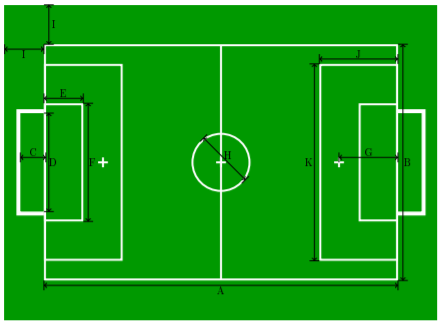
\includegraphics[scale=0.8]{images/ter.PNG}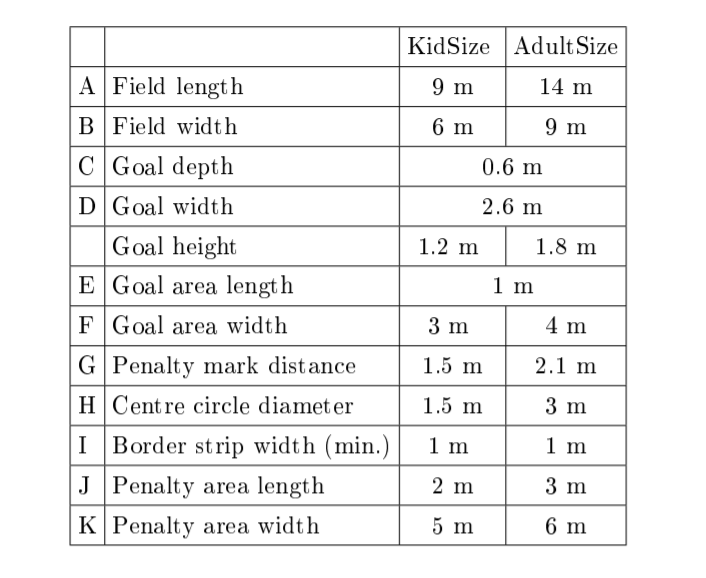
\includegraphics[scale=0.45]{images/dim_ter.PNG}
				\caption {Schéma du terrain de la roboCup avec les dimensions en catégorie Kid et Adult \cite{robocuprules} }
			\end{figure}
		}
		{Nous allons utiliser une classe \textbf{FieldModel} qui prend les dimensions du terrain en mètre, ensuite on peut représenter tous les éléments du terrain dans un repère cartésien à l'échelle que nous souhaitons.
		}{La collision avec des éléments du terrain est utilisée dans la simulation pour appliquer certaines règles : par exemple la collision de la balle et des buts.\\ }

		\item Créer les objets dynamiques de la simulation\\ \\
		Les éléments dynamiques de notre simulation sont la balle, les agents, les équipes qui manipulent des agents. Les attributs de ces éléments, l'espace d'observation des agents changent au cours de la partie à l'inverse du terrain.
		\begin{enumerate}
			\besoinVItem{Créer un agent qui représente un robot de la robocup  \textit{(Mandatory)}}
			{ On devra pouvoir donner aux joueurs des caractéristiques les décrivant, elles seront nécessaires à leurs interactions. Ces caractéristiques ne seront pas modifiées pendant le match. Ces agents
			disposent de fonctions de déplacement, de tir, de collision et d'affichage détaillées plus tard dans le rapport.

				\begin{itemize}
					\item \textcolor{olive}{Attribuer un numéro au joueur}.
					Il y a jusqu'à 4 joueurs sur le terrain. On donnera des numéros aléatoires différents de 1 à 4 aux joueurs.

					\item \textcolor{red}{Affecter le joueur à une équipe}.
					Les matchs verront s'affronter 2 équipes donc les agents seront séparés en 2 équipes A et B, de 2 couleurs différentes.

					\item Attribuer une vitesse maximum au joueur.
					Le vitesse du joueur pourra donc varier entre 0 et $borne\_sup\_v$ durant le match.

					\item \textcolor{red}{Attribuer une hitbox au joueur en forme de cercle}.
					Nécessaire pour empêcher le joueur de sortir du terrain ou tirer avec les fonctions de collisions et de tir.

					
				\end{itemize}
				Le joueur devra aussi posséder plusieurs caractéristiques décrivant son état lors du match. On les listera ci-dessous :
				\begin{itemize}

					\item \textcolor{red}{Position courante du joueur}.
					C'est la position (x,y) du joueur sur le terrain à un instant donné.

					\item \textcolor{red}{Vitesse courante en vx et vy}.
					C'est la vitesse d'un joueur à un instant donné.

					\item \textcolor{red}{Position cible du joueur.} (lors d'un mouvement).
					C'est la position qui est "ciblée" par l'agent lors d'un déplacement

				\end{itemize}

				Enfin le joueur pourra posséder des caractéristiques avancées :
				\begin{itemize}

					\item \textcolor{red}{Axe de rotation du joueur}.
					C'est l'axe de rotation en degrès par rapport à l'origine

					\item \textcolor{red}{Hitbox de tir dépendante de l'axe de rotation}.
					C'est une hitbox en cercle, elle doit translatée (être dépendante) dans le même sens que l'axe de rotation.


				\end{itemize}
			}
			{
				On a un exemple de gestion de ce genre de caractéristiques d'agents dans SlimeVolleyGym : dans le fichier slimevolley.py, avec la classe \textbf{Agent}. Pour les numéros, afin de se simplifier la tâche, on pourra les remplacer par des couleurs individuelles pour les agents ( en plus de la couleur de l'équipe) pour pouvoir les différencier notamment à l'affichage.
				Pour les caractéristiques avancées comme l'axe de rotation, on pourra s'appuyer sur des formules de trigonométrie basiques, ce code javascript par exemple effectue la rotation d'un point autour
				de l'origine. \cite{trigonometry1}.
			}
			{
				Les agents ont une place centrale dans la simulation, c'est un agent que l'on doit entraîner et c'est un agent qui doit prendre des décisions par rapport à l'espace d'actions, retourner sa perception de l'environnement en relation avec à son espace d'observations.}


			\besoinVItem{Créer l'espace d'observation  dynamique par état d'un agent}
			{	
			Il faut décrire la perception de l'agent pour pouvoir l'entrainer et lui faire prendre des décisions.
			\label{besoinObs}
				\begin{itemize}
					\item \textcolor{red}{Avoir un espace d'observation pour l'agent \textit{(Mandatory)}}
					Par défaut  l'agent percevra ses alliés, ses adversaire, la balle et les cages de but. C'est à dire que l'agent connaît à tout moment les positions des ses alliés, de la balle et des buts ennemis. On aura alors un vecteur :
					$$
					\begin{bmatrix}
						x\_agent & y\_agent & x\_allie\_agent & y\_allie\_agent \\
						x\_ennemy1\_agent & y\_ennemy1\_agent & x\_ennemy2\_agent & y\_ennemy2\_agent\\
						x\_ball & y\_ball \\
						x\_poteau1 & y\_poteau1 & x\_poteau2 & y\_poteau2 \\
					\end{bmatrix}
					\quad
					$$
					\item \textcolor{olive}{Avoir un espace d'observation dynamique \textit{(Mandatory)}} \\

					Il faut aussi que l'espace d'observation soit dynamique pour s'adapter au nombre d'agent sur le terrain tout en gardant toujours au début de la matrice les informations de l'agent à qui l'espace d'observation appartient (sinon il ne sait pas où il est par rapport aux autres).

					\item \textcolor{olive}{Activer et désactiver des paramètres dans l'observation \textit{(Optional)}}\\
					Pour pouvoir modifier l'environnement et l'apprentissage nous devons pouvoir modifier l'espace d'observation. Par exemple faire en sorte que les agents ne perçoivent plus leur adversaires ou les poteaux.\
				\end{itemize}

			}
			{
				Dans slimevolley il existe la classe \textbf{RelativeState} qui gère l'espace d'observation de l'agent, la vision de l'agent est actualisé en même temps que sa position. Ensuite l'observation d'un agent est appelé dans game.step() pour choisir une action en adéquation avec.\\
			Pour adapter la classe \textbf{RelativeState }et avoir une observation dynamique il faudrait pouvoir spécifier dans le constructeur le nombre d'agents par équipe et quels otpions font parti de la vision de l'agent et construire la matrice d'observation en fonction.

			}
			{
				Pour entrainer et faire jouer l'agent on a besoin de lui donner une perception de l'environnement.
			}

			\besoinVItem{\textcolor{violet}{Créer un équipe d'agent \textit{(Mandatory)}}}
			{Une équipe doit être composée de N agents, N allant de 1 à 11, les agents d'une même équipe doivent pouvoir se reconnaître. Dans un match 2 équipes doivent s'affronter, pour les différencier on peut leur attribuer une couleur. L'équipe a un attribut score qui lui permet de garder le nombre de but marqué par l'équipe durant le match.\label{besoinTeam}
			}
			{On a déjà créé une classe \textbf{Team} pour l'extension de slimevolley, nous allons réutiliser cette classe. Il faudrait adapter son constructeur de manière à pouvoir choisir la taille de la team et d'initialiser le bon nombre d'agents, on peut utiliser un paramètre team\_size.  }
			{On utilise l'équipe pour instancier les agents et pour les manipuler.\\
			Dans notre dernière version du code, la taille des équipes n'est pas fixée à 4 dans la classe Team, cependant les équipes sont construites uniquement avec 4 joueurs à la construction par le \textbf{GameBuilder}}.


			\besoinVItem{\textcolor{red}{Créer l'objet balle \textit{(Mandatory)}} }
			{	Il faut que la balle soit simulée par un cercle qui réagit aux tirs et rebondit lors de collisions. Elle doit avoir un diamètre de 13cm (catégorie kidsize).
				\begin{itemize}
					\item \textbf{Hitbox de la balle en forme de cercle} donnée avec le paramètre rayon.
					Pour simuler des collisions.
					\item \textbf{Position courante.}
					C'est la position (x,y) de la balle sur le terrain à un instant donné.

					\item \textbf{Vitesse courante en vx et vy.}
					C'est la vitesse de la balle à un instant donné.

					\item \textbf{Vitesse précédente en vx\_prec et vy\_prec.}
					C'est la vitesse de la balle à un instant précédent donné.
				\end{itemize}
			}{On peut réutiliser la classe \textbf{Particule} de slimevolley

			}{La balle est nécessaire pour la simulation puisque sans balle, il n'y a pas de jeux. Les agents doivent manipuler la balle pour marquer des buts\\.
			}

		\end{enumerate}

		\item Gérer les déplacements/actions des objets dynamiques

		\begin{enumerate}
			\besoinVItem{\textcolor{red}{Définir l'espace d'action d'un agent \textit{Mandatory}}}
			{L'agent a le choix parmi les actions suivantes : haut, bas, gauche, droite, tirer, tourner à droite et tourner à gauche. L'agent peut combiner des actions comme tourner et tirer ou avancer et tirer, il peut avancer en diagonale. La rotation est une canalisation (pour l'utilisateur tant que l'on appuie on tourne). L'agent a une vitesse statique. }
			{Comme dans slimeVolley, on définit l'espace d'action dans la classe \textbf{RoboCupEnv}. On déplace l'agent avec la fonction \textit{move()}, cette fonction est appelée dans  \textit{update} qui met à jour toutes les informations de l'agent. }
			{La liste d'actions représentent la liste de choix que l'agent peut faire. Pour qu'un utilisateur puisse jouer au clavier on a affecté aux actions des touches. }

			\besoinVItem{\textcolor{red}{Gérer les déplacements l'agent \textit{Mandatory}}}
			{
				Il faut simuler les déplacements de l'agent, en effet celui-ci dispose d'un axe de rotation, il doit pouvoir avancer, reculer, translater à gauche, translater à droite.	\\

			}
			{Pour cela, on utilisera des formules de trigonométrie \cite{trigonometry2} pour retrouver les coordonnées d'un point après translation d'une distance (vitesse x, y dans le repaire cartésien) par rapport à l'angle de rotation depuis l'origine.}
			{}


			\besoinVItem{\textcolor{red}{Gérer les déplacements de la balle \textit{Mandatory}}}
			{
				Il faut simuler le déplacement de la balle. Les joueurs et les lignes du terrain doivent pouvoir interagir avec. Lorsque la balle est en mouvement elle ralentie et finit par s'arrêter. Les agents peuvent tirer dans la balle ou "dribbler"\footnote{On utilise ce terme quand les agents font avancer la balle en la poussant } avec. La balle rebondit sur les poteaux.	\\
				On pourrait aussi rajouter les frottements de la balle avec l'herbe en fonction du sens de picots de l'herbe synthétique \textit{(Optional)}.
			}
			{Pour simuler le rebondissement de la balle sur les poteaux, on utilise une fonction de collision naîve qui détecte la collision entre un rectangle et un cercle \cite{collision1} , pour le rebondissement on applique la vitesse opposée}
			{L'agent tir et donne une vitesse et une accélération à la balle. La fonction move() va ensuite déplacer le ballon à chaque tour de boucle de simulation.}

			\besoinVItem{Contraintes de déplacements : balle et terrain}
			{Certains déplacements sont interdits.
				\begin{itemize}
					\item \textcolor{red}{Rester sur le terrain (balle) \textit{Mandatory}} La balle ne doit pas pouvoir sortir à l'extérieur du terrain\footnote{Elle ne doit pas franchir les lignes de touches}.
					\item \textcolor{red}{Rester dans la fenêtre (agent) \textit{Mandatory}} L'agent doit rester dans la fenêtre.
					\item \textcolor{violet}{Rester sur le terrain (agent) \textit{Important}} L'agent ne doit pas pouvoir sortir des lignes du terrain.
					\item \textcolor{red}{Respecter le placement de début de match \textit{Mandatory}} Au début du match chaque équipe doit être dans sa moitié de terrain.
				\end{itemize}
			}
			{Pour contrôler les déplacements des agents et de la balle on vérifie si le déplacement qu'ils souhaitent faire est autorisé s'il ne l'ait pas, on n'exécute pas l'action/déplacement en mettant la vitesse à 0 notamment avec la méthode cancel\_movement. \\
			Pour le positionnement des agents au début du match on passe par le constructeur de l'agent et on lui donne une position valide. On pourrait aussi faire une fonction qui gère le placement des agents automatiquement en fonction de leur nombre.
			}
			{Les déplacements sont vérifiés lorsque l'on déplace les objets. S'il faut restreindre un déplacement fonction on appelle \textit{cancel\_movement} qui est appelée dans \textit{update} pour l'agent. \\}

		\end{enumerate}
		\besoinVItem{\textcolor{red}{Gérer la collision entre agents \textit{Mandatory}}
		}
		{Il faut implémenter une collision entre agent sinon les agents peuvent se traverser. Les agents n'ont pas besoin de rebondir il faut juste qu'ils se bloquent le passage.
		}
		{On a déjà implémenté la collision entre agent d'une même équipe dans slimevolley, il faut adapter cette collision pour qu'elle concerne tous les agents. Pour l'instant nous avons une méthode naïve qui vérifie la collision entre 4 agents. Pour gérer les collisions on a créé une nouvelle classe \textbf{Referee} qui fera office d'arbitre. La méthode \textit{update\_referee()} est appelée dans \textbf{Game} à chaque pas de temps du jeu.
		}
		{La collision entre agents est appelée à chaque pas de temps dans la boucle de la simulation. On va aussi créer une option qui pénalise la collision, ce sera une des fautes de jeu. \\ }
		\item Afficher les éléments de la simulation
		\begin{enumerate}
			\item Mise à l'échelle par rapport à la fenêtre
			\begin{enumerate}
				\besoinVItem{\textcolor{red}{Convertir les coordonnées du repaire cartésien en coordonnées de la fenêtre \textit{Important}}
				}
				{On doit pouvoir convertir les données du repaire cartésien de la simulation robocup qui est plus petit que la taille réelle de
				la fenêtre.

				}
				{On utilise pour cela une classe \textbf{Window} qui applique un facteur d'agrandissement aux coordonnées x, y d'une entité,
					au rayon d'un cercle, à la largeur et la hauteur d'un rectangle.
				}
				{}

			\end{enumerate}

			\item Afficher des formes géométriques

			\begin{enumerate}
				\besoinVItem{\textcolor{red}{Afficher des cercles et des rectangles \textit{Important}}
				}
				{Pour représenter nos éléments du terrain, il suffit d'afficher des cercles et des rectangles.

				}
				{On utilise une bibliothèque externe, le package \textit{rendering} de la bibliothèque gym, qui utilise un autre package populaire de rendu graphique en python \textit{pyglet}, celui-ci nous permet de créer des canvas facilement. De la même manière que SlimeVolley.
				}
				{}

			\end{enumerate}


			\item Afficher le terrain
			\begin{enumerate}
				\besoinVItem{\textcolor{red}{Afficher tous les éléments du terrain \textit{Important}}
				}
				{On doit pouvoir afficher les lignes de touche, les cages de but, la zone de but, la ligne du milieu, le cercle du milieu.

				}
				{On récupère pour cela les données de la classe \textbf{FieldModel} et on effectue une conversion des coordonnées à l'échelle de la
				fenêtre (on fait de même pour tous les autres affichages). On utilise le module \textit{rendering} pour créer des rectangles, pour se simplifier la tâche, limiter le nombre de canvas et donner l'impression que l'on affiche des lignes, on dessine à la fois un rectangle blanc puis un rectangle à l'intérieur avec la couleur de la pelouse du terrain.
				}
				{On peut vérifier si lorsque la balle du terrain visuellement, le modèle spécifie que la balle sort effectivement du terrain dans
				le repère cartésien.}

			\end{enumerate}



			\item Afficher les équipes d'agents
			\begin{enumerate}
				\besoinVItem{\textcolor{red}{Afficher tous les agents \textit{Important}}
				}
				{On doit pouvoir afficher les éléments, agents du terrain, afficher leur couleur d'équipe, mais également leur couleur secondaire pour pouvoir les reconnaître en tant qu'agent individuellement.

				}
				{On récupère pour cela les agents dans les équipes \textbf{Team}, les informations associées (couleur d'équipe, couleur individuelle) les coordonnées. On utilise des cercles pour dessiner les agents avec le module \textit{rendering}.

				}
				{}

				\besoinVItem{\textcolor{red}{Afficher les yeux des agents \textit{Optional}}
				}
				{On doit pouvoir afficher les yeux des agents, cela peut nous permettre facilement de vérifier que la rotation fonctionne.

				}
				{On récupère les coordonnées des yeux dans la classe \textbf{Agent}, ces données sont mis à jour à chaque fois que l'on appelle la
				méthode update().
				}
				{On peut vérifier si les yeux sont bien translatés par rapport à l'axe de rotation}

				\besoinVItem{\textcolor{red}{ Afficher la hitbox des agents \textit{Optional}}
				}
				{On doit pouvoir afficher la hitbox des agents, cela peut nous permettre facilement de vérifier que le tir est dépendant
				de l'axe de rotation.

				}
				{On récupère les coordonnées de la hitbox dans la classe \textbf{Agent}, ces données sont mis à jour à chaque fois que l'on appelle la
				méthode update().
				}
				{On peut regarder si le tir est possible lorsque la balle est en collision avec la hitbox}
			\end{enumerate}
			\item Afficher la balle

			\begin{enumerate}
				\besoinVItem{\textcolor{red}{Afficher la balle dans le terrain \textit{Important}}
				}
				{Il est nécessaire d'afficher la balle pour la simulation robocup.

				}
				{On récupère les coordonnées de la classe \textbf{Ball} et on dessine un cercle.
				}
				{}

			\end{enumerate}

			\item  Récupérer les données des différents modèles à chaque cycle d'exécution


			\begin{enumerate}
				\besoinVItem{\textcolor{red}{Récupérer les données du terrain, des équipes, de la balle \textit{Important}}
				}
				{Il est nécessaire de récupérer ces données à chaque mis à jour.

				}
				{La classe RoboCupEnv transmet automatiquement à l'objet \textbf{View} les données nécessaires.
				}
				{. \\}

			\end{enumerate}


		\end{enumerate}

		\item Définir toutes les règles de la simulation
		\begin{enumerate}
			\besoinVItem{\textcolor{violet}{Définir les fautes et pénalités associées \textit{Important}}
			}
			{Les fautes seront optionnels dans l'environnement, on aura la collision entre agent, les erreurs de placements des agents (sortir du terrain, être mal positionné en début de jeu), et les sorties de balle. Pour pénaliser les fautes nous avons prévus ces pénalités.
				\begin{itemize}
					\item Collision entre agents ou erreurs de placement :
					\subitem Exclure les agents temporairement : pour cette pénalité il faut autoriser les agents à aller sur le banc de touche  pendant la durée de la pénalité, ensuite il faut définir un point d'entré sur le terrain pour qu'il retourne jouer.
					\subitem Immobiliser les agents (simuler le fait que l'agent soit tombé et se relève)
					\subitem Donner la balle à l'équipe adverse
					\item Sortie de Balle :
					\subitem Donner la balle à l'équipe adverse
				\end{itemize}
			}
			{Les fautes collision, sortie de balle ont déjà été expliquées dans le besoins au dessus. Il faut maintenant que les fautes soient associées à une pénalité. Pour cela nous allons utiliser \textbf{Referee}. Pour donner la balle à l'équipe qui ne l'a pas sortie il faut créer un champ \textit{last\_touched} qui garde en mémoire l'équipe qui a touchée la balle en dernier. Ensuite pour donner la balle à l'autre équipe on doit créer une nouvelle phase de jeu. On peut faire en sorte qu'un agent tir la touche ou on pourrait revenir en position d'engagement avec la fonction \textit{new\_Match} le match en donnant la balle à la bonne équipe.\\
			Pour immobiliser l'agent on pourrait lui affecter un champ immobile que \textbf{Referee} gérerait, avec le champ à true les déplacements serait désactiver avec la fonction \textit{cancelled\_movement}.
			}
			{Les fautes et pénalités sont activées à la création d'un environnement, ensuite elles ont un impact sur le déroulement du match et le déplacements des agents.\\
			Nous avons implémenté les fautes collision et sortie de la balle, par contre nous n'avons pas implémenté de pénalités. }


			\besoinVItem{\textcolor{violet}{Créer les phases de jeu}
			}
			{Pour la gestion d'un match il faut implémenter différentes phase de jeu qui ont des contraintes spécifiques. Voila la listes des phases de jeu :
				\begin{itemize}
					\item \textcolor{red}{Engagement \textit{Mandatory} } il faut que les éléments de la simulation ait une position de départ. Les agents sont de chaque coté de leur terrain, la balle est au centre.
					\item \textcolor{red}{En jeu \textit{Mandatory} } durant cette période les agents jouent.
					\item \textcolor{red}{Marquer un but \textit{Mandatory} } après un but on doit mettre à jour le score des équipes et reset le match pour revenir à la phase d'engagement.
					\item \textcolor{red}{Fin du match \textit{Mandatory} } il faut que le match puisse s'arrêter pour cela on met en place un timer.
					\item \textcolor{olive}{Arrêt de jeu : Faute \textit{Optional} } pour gérer les fautes a besoin de faire des arrêt de jeux par exemple si on veut faire tirer une touche à un agent.

				\end{itemize}
			}
			{Pour l'engagement on adapte la fonction \textit{new\_match} de slimevolley. Dans l'environnement Gym on a le champ done de \textit{step} qui renvoie true si le match est terminé. Pour marquer un bur on a juste a ajouter +1 au score de \textbf{Team}.
			}{Les phases de jeu sont appelées dans la classe \textbf{Game} en fonction de ce qu'il se passe sur le terrain. \\
			}

		\end{enumerate}

		\item Faire l'interfaçage avec l'abstraction d'un environnement Gym \\

		Gym fournit principalement une abstraction de la représentation d'un environnement avec l'interface Env, il faut donc implémenter cette interface pour pouvoir créer un
		environnement et interagir avec celui-ci , respecter les consignes de la documentation  pour qu'il soit correctement interprétable par les
		différents algorithmes disponibles dans la bibliothèque stable\_baselines.\\
		En revanche, Gym laisse la liberté à l'utilisateur de représenter un agent de la manière dont il souhaite, il n'y a pas de restrictions. \\

		\begin{enumerate}
			\besoinVItem{\textcolor{red}{Construire l'espace d'observations par défaut \textit{Mandatory}}
			}
			{Il faut construire l'espace d'observations pour l'environnement par défaut (KidSize ou AdultSize)
			}
			{Il faut définir l'attribut observation\_space. Il est nécessaire d'utiliser l'objet \textit{Space} de la bibliothèque gym, pour que l'on puisse correctement faire fonctionner
			les différents algorithmes d'apprentissage de bibliothèque stable-baselines.

			Cet espace est représenté par un objet de type \textit{Box} (implémentation de la classe Space du module gym), cet espace représente une "boîte" à n dimensions.
			Ici, chaque paramètre de la matrice à un intervalle de valeurs acceptées (valeurs basses et hautes).\\

			Ce mode d'observation est utilisé dans l'environnement SlimeVolley-v0.

				\begin{center}
					\begin{tabular}{ |c|c|c|c|c|c| }

						\hline
						observation    & $x\_agent$ & $y\_agent$ & $\dot{x} \_agent$ & $\dot{y} \_agent$ & ...\\
						min & -3.4028235e+38 & -3.4028235e+38 & -3.4028235e+38 & -3.4028235e+38 & ...\\
						max & 3.4028235e+38 & 3.4028235e+38 & 3.4028235e+38 & 3.4028235e+38 & ...  \\
						\hline
					\end{tabular}
				\end{center}

				Dans l'environnement par défaut, sans masquage de la vision de l'allié et des adversaires, celui-ci doit être de taille 20. Positions(x, y), vitesse(x, y), donc 4 paramètres pour les 4 agents(16), puis la balle(20).
			}
			{}

			\besoinVItem{\textcolor{red}{Adapter l'espace d'observations lorsque l'on masque des éléments \textit{Important}}
			}
			{Il est nécessaire d'adapter l'espace d'observations lorsque l'on masque la vision de l'allié ou des ennemis.
			}
			{Une grande partie du travail consiste à adapter la classe \textbf{RelativeState} pour qu'elle puis être modulaire. Sinon, au niveau de l'environnement gym il suffit juste de changer la taille de la matrice, 16 si on masque la vision de l'allié, 12 si on masque la vision des adversaires, 8 si on masque la vision de l'allié et des adversaires.
			}
			{}

			\besoinVItem{\textcolor{red}{Adapter l'espace d'actions \textit{Mandatory}}
			}
			{Il faut définir l'attribut action\_space. Il est nécessaire d'adapter l'espace d'actions, pour pouvoir prendre en compte les 7 actions possibles, translater à gauche, translater à droite, avancer, reculer, tirer, tourner à gauche, tourner à droite.
			}
			{On réutilise le même espace d'actions que l'environnement SlimeVolley-v0.
			Dans le mode MultiBinary on a un espace d'actions représenté par un vecteur de booléens à 3 dimensions avec les champ avancer, reculer, sauter (droite, gauche, haut). La valeur est à 1 si l'action est demandée, 0 dans le cas contraire. \\
			Pour la version robocup il suffit d'augmenter la taille de ce vecteur en passant à 7.
			}
			{}

			\besoinVItem{\textcolor{olive}{Adapter l'espace d'actions lorsqu'on réduit les actions possibles. \textit{Optional}}
			}
			{Il est nécessaire d'adapter l'espace d'actions, si l'on souhaite désactiver, le tir ou la rotation.
			}
			{Il suffit simplement de changer la taille du vecteur, 5 dans le cas où on désactive la rotation, 6 dans le cas où on désactiver le tir,
				4 dans le cas où on désactive le rotation et le tir.
			}
			{}

			\besoinVItem{\textcolor{red}{Renvoyer des informations sur l'état de l'environnement après l'exécution de plusieurs actions. \textit{Mandatory}}
			}
			{Il faut pouvoir récupérer les observations de l'agent que l'on entraîne, sa récompense, une information pour indiquer si le jeu est terminé.
			}
			{Dans le modèle gym la méthode step(action), retourne des informations sous la forme d'un tuple obs=object, reward=float, done=bool.
			Les observations de l'agent entraîné sont récupérées sous la forme d'une numpy array, la récompense est renvoyée selon la perspective de l'agent que l'on entraîne, résultat positif si son équipe a marqué un point, négatif si l'équipe adverse a marqué un point, nul si la balle est toujours en jeu, la condition d'arrêt done à vrai si une équipe a marqué 5 points, ou si 10 minutes se sont écoulés. Ces informations sont renvoyées par la classe \textbf{Game}.
			}
			{}

			\besoinVItem{\textcolor{red}{Pouvoir choisir dynamiquement l'agent que l'on entraîne à la création de l'environnement \textit{Important}}
			}
			{On souhaite pouvoir choisir dynamiquement l'agent que l'on entraîne. Dans le modèle d'apprentissage de gym, lorsqu'on appelle step(action, *args), seulement la première action est prise en considération dans la plupart des modèles (par exemple PPO). On, souhaite donc pouvoir choisir à quel agent il faut attribuer cette action parmi les 4. Il faut également pouvoir récuper les observations de ce dernier.
			}
			{Lorsque l'on crée un environnement RoboCupAdultSize-v0 ou RoboCupKidSize-v0, on peut répartir les actions entre les agents, on fait une \{association couleur\_agent = numéro\_action\_step\}. La classe \textbf{Game} reconnaît l'agent que l'on entraîne et retourne des observations de celui-ci. La classe \textbf{Team} prend en considération le numéro des actions lorsqu'elle demande aux agents d'exécuter telle action.
			}
			{}

			\besoinVItem{\textcolor{red}{Récuper les observations des autres agents (que l'on entraîne pas) \textit{Important}}
			}
			{On souhaite pouvoir récupérer les observations par états des autres agents, ce qui peut être utile pour le débugage.
			}
			{Il faut renvoyer depuis step un dictionnaire info qui est d'ailleurs optionnel, on peut y inclure des associations {couleur\_agent : matrice d'observation par états}.
			}
			{}

			\besoinVItem{\textcolor{red}{Réinitialiser l'environnement \textit{Mandatory}}
			}
			{On souhaite pouvoir réinitialiser l'environnement à son état initial, avant que toutes les actions soient exécutées.
			}
			{Il est nécessaire de réintialiser l'environnement en implémentant la méthode reset() de l'interface \textbf{Env} de la bibliothèque gym.
			Pour cela, on peut simplement effectuer une copie récursive de l'objet Game à son état initial. On peut utiliser la bibliothèque copy en python.
			}
			{}

		\end{enumerate}

	\end{enumerate}

	\subsubsection{Pouvoir entrainer un agent dans nos différents environnements robocup}
	L'extension slimultiagent est une preuve de concept pour l'apprentissage par renforcement multi-agents. Les besoins énoncés ci-dessous ont seront implémentés dans la partie robocup mais ils ont été détaillés lors de l'analyse des besoins sur SlimeVolleyGym multiagent 2vs2. Nous avons seulement du adapter ces besoins pour la robocup et ils ne représenteront pas de défis techniques plus complexes. C'est pourquoi on énoncera seulement les besoins pour pouvoir entrainer un agent dans les différents environnements robocup et on renverra le lecteur à la partie dans slimultiagent qui détail le point en particulier.
	\begin{enumerate}
		\item Lancer une session d'entrainement dans l'environnement robocup (cf \ref{session})
		\item Avoir un algorithme opposant contre qui entrainer un agent (cf \ref{opposant})
		\item Sauvegarder les données d'un apprentissage  et pouvoir les réutiliser (cf \ref{sauvegarde})
		\item Récupérer les résultats d'un match et d'un entrainement (cf \ref{résultats})
	\end{enumerate}
	\subsubsection{Pouvoir paramétrer un environnement robocup et les comportements des agents}
	\begin{enumerate}
		\item \textcolor{red}{Pouvoir choisir avec un JSON les paramètres d'un environnement \textit{Mandatory}}\\
		Au moment de lancer le script voulu, il ne faut plus contrairement au code de Hardmaru, donner les paramètres
		en ligne de commande. Il suffit maintenant de les mettre aux champs correspondants dans un seul fichier JSON.

		\item Générer l'environnement à partir du fichier JSON\\
		Grâce à notre librairie, le script peut aller chercher les paramètres nécessaires à la fabrication
		de l'environnement à l'aide d'une fonction d'accès aux données dans le JSON.
		Gym génère ensuite l'environnement avec les éléments ainsi retournés.

		\item Faire en sorte que les paramètres choisis soient compatibles.\\
		Si un paramètre est lointain dans les objets, la récupération de la donnée se fait dynamiquement
		et surtout sans utiliser d'accès incessants au même fichier de données.
		Il faut néanmoins donner par exemple des paramètres de configuration existants comme documenté
		dans le README.

		\item Choisir la politique des teams à partir d'un fichier JSON
		L'un des grands avantages à cette stratégie d'utilisation d'un JSON est que l'on peut modifier
		la liste des ia des équipes directement dans le fichier, ce qui apporte une grande praticité et surtout
		flexibilité pour ce qui est de lancer des évaluations entre intelligences artificielles.
	\end{enumerate}

	\subsubsection{Pouvoir évaluer l'efficacité de stratégies dans différents environnements Robocup et contre diverses stratégies }
	\begin{enumerate}
		\item \textcolor{violet}{Récupérer le résultat d'un match, les politiques qui se sont
		affrontées et l'environnement dans lequel il s'est déroulé \textit{Mandatory}}\\
		Pour se faire, on écrit dans un fichier de résultats csv comportant le nom de l'environnement,
		qui va contenir l'ensemble des scores entre deux modèles entraînés ainsi que les autres.
		Notre librairie différencie les résultats contre soi-même dans le fichier finissant par
		'selfplay' et celui contre les autres ne contenant pas 'selfplay', cela pour obtenir et
		comparer des résultats cohérents entre eux. Si l'on fait fait jouer d'autres modèles venant
		d'autres ia dans un même environnement, les résultats ainsi que les noms vont s'additionner
		dans le même fichier à la suite des précédants résultats et dans le champ des noms.

	\end{enumerate}



	\section{Architecture logicielle}

	\subsection{Diagramme de classes}
	Nous allons maintenant vous présenter l'architecture globale de notre application.
	Nous avons utilisé des patterns d'architecture tel que MVC ou le Builder. Nous avons décidé de la présenter en quatre parties :
	premièrement l'interface avec l'environnement Gym, deuxièmement la création de la classe \textbf{Game} qui est aggrégé par la classe \textbf{RoboCupEnv}
	de l'environnement Gym, troisièmement la partie métier de notre application et pour finir le fonctionnement de la classe \textbf{RelativeState} qui s'occupe de l'espace d'observations de l'agent.\\

	\subsubsection{Interface avec l'Environnement Gym}

	\begin{figure}[H]
		\centering
		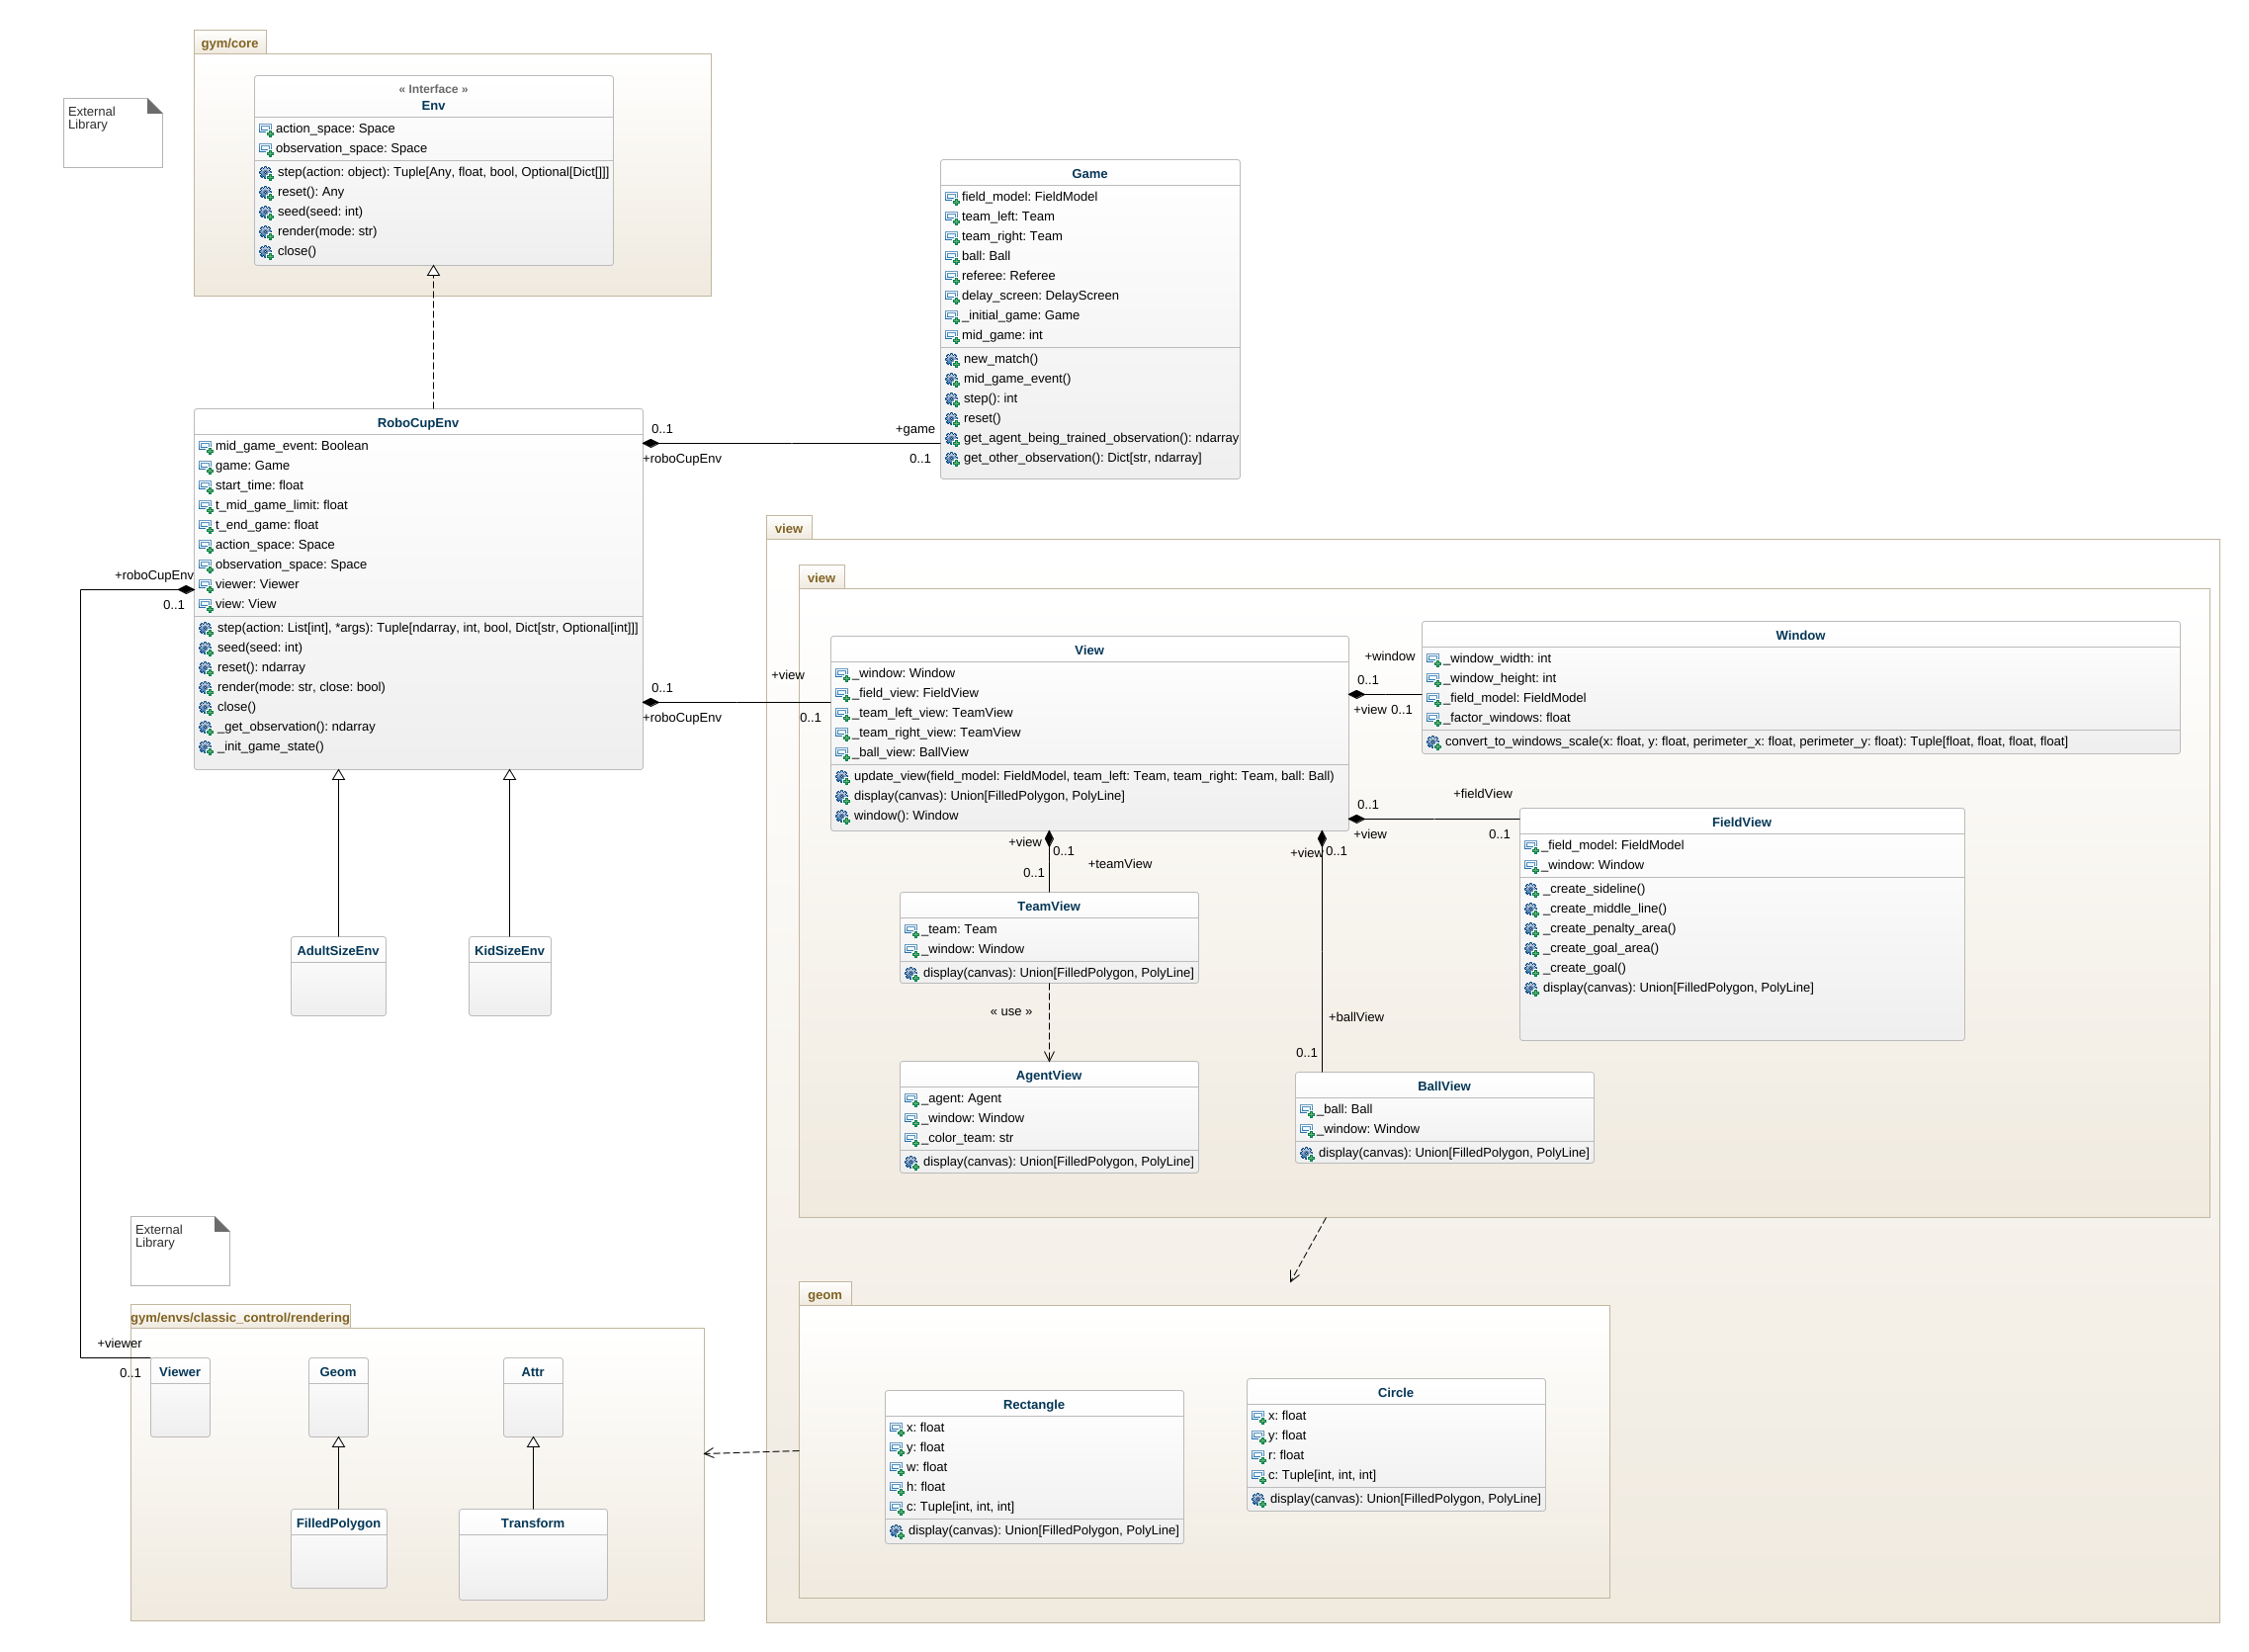
\includegraphics[scale=0.30]{images/robocup-env.png}
		\caption {Diagramme de classes: Interface avec l'Environnement Gym  }
	\end{figure}

	Cette partie du diagramme de classes regroupe les classes qui interagissent avec l'environnement gym,
	la classe \textbf{RoboCupEnv} implémente l'interface \textbf{Env} du package gym, les classes héritantes (\textbf{AdultSizeEnv}, \textbf{KidSizeEnv})
	créent un jeu (\textbf{Game}) d'une manière différente.
	La classe \textbf{Game} est une classe qui agrège tous les composants cœurs de l'environnement (les équipes, la balle, le terrain, l'arbitre), elle interagit avec l'environnement
	en exécutant les actions demandées et en renvoyant les données d'observations pour chacun des agents.
	On ne le voit pas dans le diagramme, mais la méthode reset() de \textbf{Game} est implémentée de la même manière qu'un \texttt{Prototype} (design pattern), en clonant
	le jeu à l'état initial (avant toutes les éxécutions des actions). \\
	Ce diagramme est semblable au pattern \texttt{Model View Controller}, on a choisi de séparer les traitements relatifs à la vue, du modèle, afin de ne pas
	mélanger les données de la vue et du modèle, la classe
	\textbf{RoboCupEnv} fait office de contrôleur, on peut exécuter des actions sur l'environnement sans pour autant afficher la vue.
	\\
	\noindent Limitations : \\
	\begin{itemize}
		\item Le contrôleur (\textbf{RoboCupEnv}) n'effectue pas vraiment d'actions de contrôle à part activer/désactiver la vue.
	\end{itemize}


	\subsubsection{Création}

	\begin{figure}[H]
		\centering
		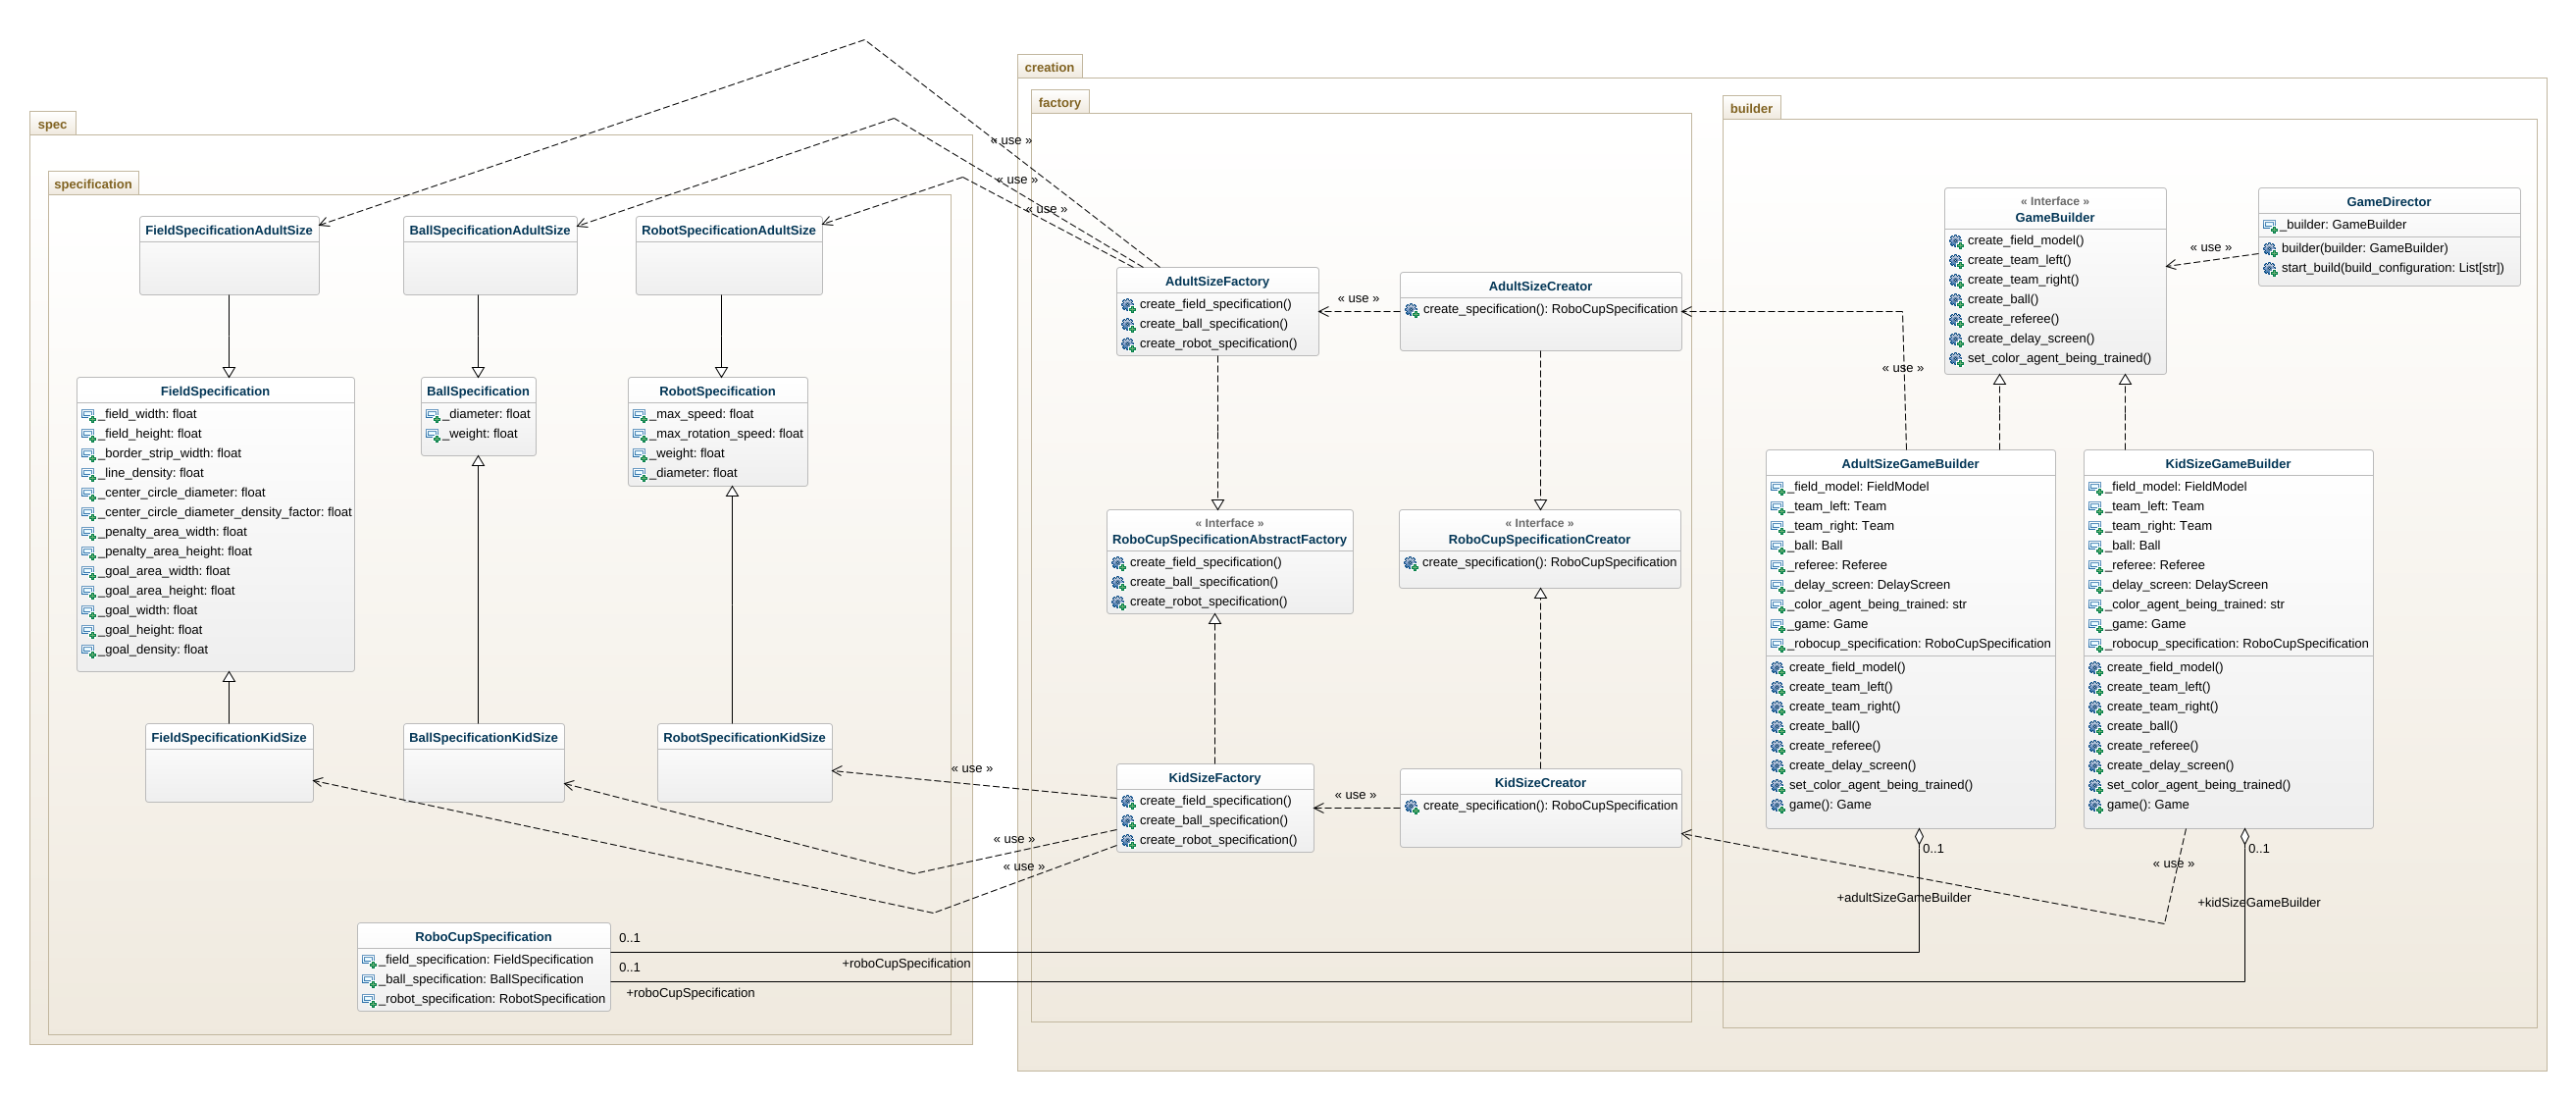
\includegraphics[scale=0.26]{images/robocup-creation.png}
		\caption {Diagramme de classes: Création  }
	\end{figure}

	On a choisi d'isoler complétement le processus de création de l'objet \textbf{Game}, qui est un objet complexe et configurable, on a pour cela
	utiliser le design pattern \texttt{Builder}. En effet, les classes \textbf{AdultSizeEnv} et \textbf{KidSizeEnv} font appel à classe \textbf{GameDirector} en plaçant le Builder approprié, celui-ci va lancer l'exécution de la création du jeu en suivant des étapes précises de construction. \\
	La différence principale entre la classe \textbf{AdultSizeGameBuilder} et \textbf{KidSizeGameBuilder} c'est qu'ils ne travaillent pas avec les mêmes données de spécification, celles-ci représentent les valeurs réelles des éléments de la RoboCup (les dimensions du terrain, la taille de la balle et des agents par exemple). \\ La création des données de spécification est déléguée aux classes de création implémentant l'interface \textbf{RoboCupSpecificationCreator} (pattern \texttt{method factory}), ces sous-classes re déléguent la construction à une fabrique abstraite (\textbf{RoboCupSpecificationAbstractFactory}) (pattern \texttt{abstract factory}), les familles d'objets sont les données de spécification de type KidSize et celles de type AdultSize. \\
	Cette architecture permet une certaine modularité dans la création d'un jeu. \\
	\\
	\noindent Limitations : \\
	\begin{itemize}
		\item Le code des classes \textbf{AdultSizeGameBuilder} et \textbf{KidSizeGameBuilder} ne diffère que d'une ligne, à la création des spécifications, le code est dupliqué, cependant, on a souhaité laisser le code en l'état dans l'optique où l'on souhaiterait vraiment rajouter des traitements différents.
		\item La classe \textbf{GameDirector} devrait proposer plus de configurations de construction possibles (placement des joueurs par exemple).
	\end{itemize}

	\subsubsection{Cœur de l'environnement}
	\newpage
	\begin{figure}[H]
		\centering
		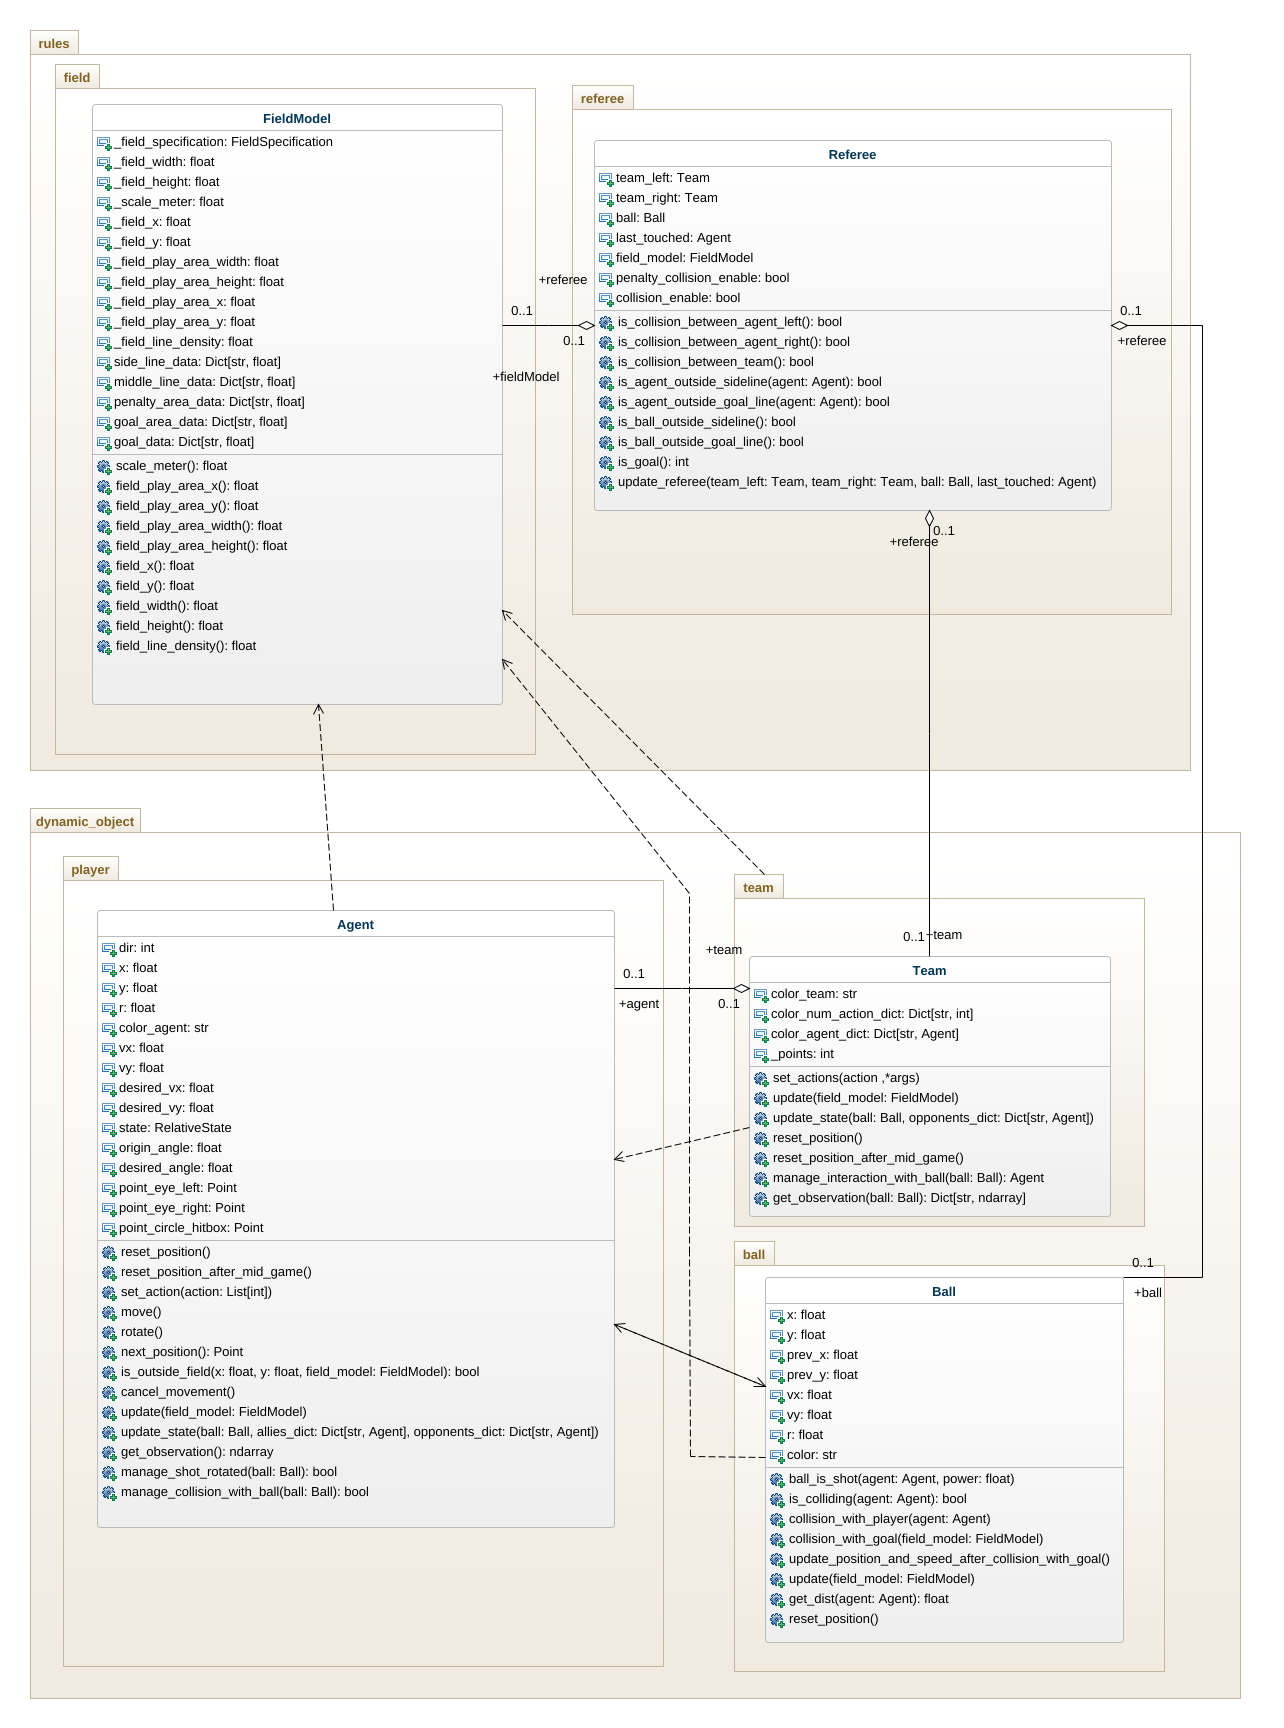
\includegraphics[scale=0.5]{images/robocup-core.png}
		\caption {Diagramme de classes: Coeur de l'environnement  }
	\end{figure}

	Cette partie du diagramme regroupe les éléments qui exécutent les traitements métiers principaux. Toutes les classes dépendent
	de la classe \textbf{FieldModel}, celle-ci permet de représenter le repaire cartésien du terrain, et donc les coordonnées possibles des agents.
	Elle crée ses données à partir d'une classe \textbf{FieldSpecification}, elle reproduit les mêmes traitements de calcul des coordonnées des différents éléments du terrain(lignes de touche, cages de but) que le terrain soit en AdultSize ou en KidSize. \\
	La classe \textbf{Referee} permet d'arbitrer les agents, ces principaux traitements concernent la gestion des déplacements des agents (ne pas sortir du terrain), vérifier également que la balle a atteint ou non la cage d'un but, retourner le résultat. Elle aggrège donc les deux équipes, la balle et le terrain. \\
	La classe \textbf{Team} représente des équipes d'agents, ces traitements concernent l'éxécution des actions sur les agents de l'équipe, mettre à jour
	la position, l'état relatif, récupérer les données d'observation par états, réinitialiser les positions (en cas de point ou à la mi-temps), de chacun des agents. \\
	Pour la classe \textbf{Agent}, on retrouve des caractéristiques classiques d'un jeu en 2D (mettre à jour sa position dans le repaire cartésien après avoir effectué un déplacement, faire une rotation avec un certain angle par rapport à l'origine). Cependant, dans le cadre
	de l'apprentissage par renforcement on y incorpore des traitements supplémentaires pour pouvoir mettre à jour l'état relatif de l'agent, exécuter des actions de l'environnement, récupérer les données d'observation par états.\\
	Pour la classe \textbf{Ball}, on retrouve principalement des traitements pour mettre à jour la position en fonction de la vitesse, vérifier
	si la balle est collision avec les poteaux des buts, avec le joueur. La balle n'est pas un agent donc elle ne dispose pas de données d'obervations.\\

	\noindent Limitations : \\
	\begin{itemize}
		\item L'attribution du rôle des classes n'est pas assez logique, on retrouve des traitements qui devraient être situé dans d'autres classes, par exemple pour la méthode is\_outside\_field de la classe \textbf{Agent} qui devrait être situé dans la classe \textbf{FieldModel}.
		\item Problème de dépendances circulaires, par exemple la classe \textbf{Ball} dépend de la classe \textbf{Agent} et inversement.
		\item La classe \textbf{Agent} regroupe trop de fonctionnalités, on aurait souhaité implémenter le pattern \texttt{Decorator}, pour permettre une modularité dans le choix des caractéristiques principales des agents (tourner, accélérer). Cependant, l'état de cette classe est
		accédé dans plusieurs autres classes (récupération des coordonnées et des vitesses) au lieu d'avoir des fonctionnalités métiers, on ne pouvait donc pas créer d'interface sans devoir effectuer un grand refactoring.
	\end{itemize}

	\subsubsection{Représentation de l'observation de l'agent}

	\begin{figure}[H]
		\centering
		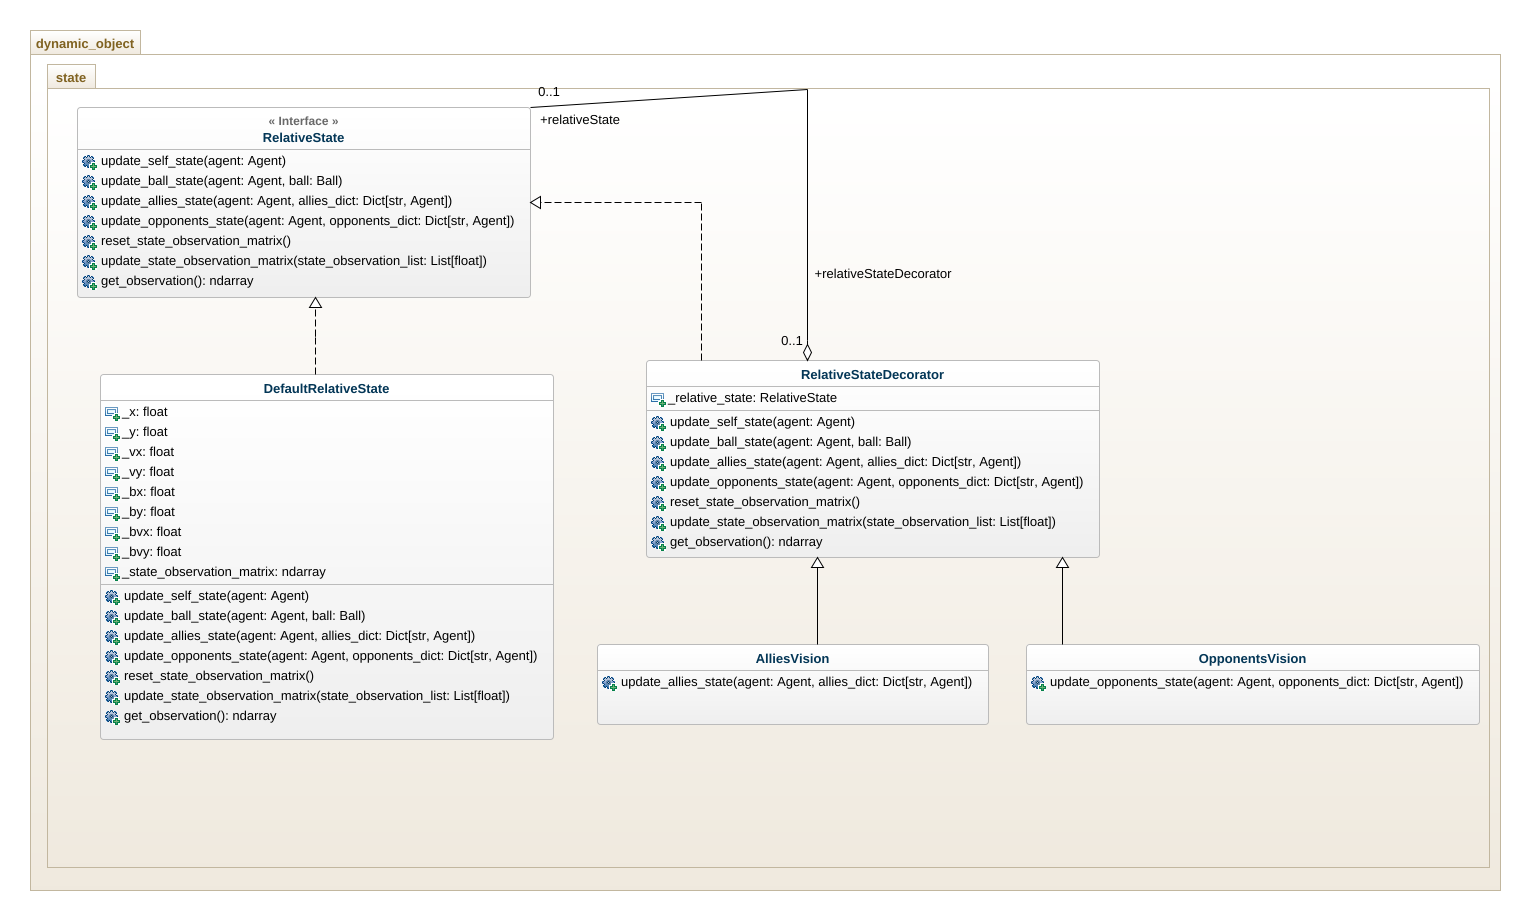
\includegraphics[scale=0.46]{images/robocup-state.png}
		\caption {Diagramme de classes: Représentation de l'état relatif}
	\end{figure}

	Ce diagramme de classe représente la manière dont on a implémenté l'état relatif de chacun des agents (la matrice d'observations par états).
	La classe concrète \textbf{DefaultRelatifState} représente l'espace d'observations de base sans extensions (l'agent voit uniquement son propre état et celui de la balle, les observations des alliés et des opposants sont masquées). On a principalement des traitements pour mettre à jour, réinitialiser l'espace d'observations et récupérer les données associées. Afin de gagner en souplesse, on a utilisé le design pattern \texttt{Decorator}, en effet, les classes \textbf{AlliesVision} et \textbf{OpponentsVision} "décorent" le composant concret \textbf{DefaultRelatifState} en rajoutant les données d'observations des alliés et/ou des opposants. Il n'est pas nécessaire de créer une autre classe qui effectue à la fois l'ajout des observations des alliés et des opposants. \\
	L'avantage de ce pattern, c'est que l'on pourrait facilement rajouter les observations des poteaux des cages de but. \\

	\noindent Limitations : \\
	\begin{itemize}
		\item L'interface \textbf{RelatifState} limite les possibilités d'espaces d'observations en fixant le type en une numpy array.
	\end{itemize}


	\subsection{Bibliothèques utilisées}

	\begin{itemize}
		\item numpy \cite{numpy}: on s'en sert principalement pour créer les espaces d'observation par états des agents.
		\item gym \cite{openaigym}: ce package nous permet de faire l'interface avec l'environnement gym (module core), représenter nos données d'observations
		avec l'objet \textbf{Space} (package spaces), utiliser le module rendering pour effectuer le rendu du jeu en utilisant une bibliothèque graphique.
		\item colour: c'est un package qui nous permet de faire des conversions de couleurs en chaîne de caractère en valeurs rgb facilement.
		\item pyglet: c'est un package de rendu graphique, le module rendering de gym dépend de celui-ci
		\item parameterized \cite{parameterized} permet d'écrire des tests plus facilement, le paramètrage des tests est possible
		\item abs: package qui nous permet de rajouter des annotations au code pour spécifier qu'une méthode est abstraite par exemple.
		\item typing \cite{typing}: package qui nous permet d'annoter le typage en python pour faciliter la lecture et la compréhension du code (le typage reste cependant dynamique).
		\item copy \cite{copy}: ce package nous permet d'effectuer des copies d'objets facilement (semblable au pattern \texttt{Prototype}.
		\item unittest \cite{unittest}: bibliothèque de tests unitaires

	\end{itemize}



	\section{Fonctionnement de l'application}
	Notre application est composée de trois parties. Ces différentes parties définissent les différentes étapes allant de la création et de la modification de l'environnement de jeu à l'évaluation des différents résultats d'entraînement pour un type d'algorithmes spécifique. Ces parties sont :
	\begin{itemize}
		\item Test en mode manuel (seul un humain peut jouer) qui permet après l'implémentation de nouvelles fonctionnalités de les tester en bougeant manuellement deux équipes de deux joueurs.
		\item Un mode entraînement qui va entraîner un agent via un algorithme implémenté par l'utilisateur et généré des résultats (au format JSON) exploitable par le mode évaluation.
		\item Le mode d'évaluation qui permet d'évaluer l'entrainement d'un agent en le faisant affronter contre un autre agent choisi par l'utilisateur.
	\end{itemize}

	\subsection{Le mode manuel}
	Le mode manuel comme présenter plus haut permet de tester via le clavier l'interface de jeu dans un environnement basique.
	Les paramètres de jeu sont définis dans le fichier env.json disponible dans le répertoire src/robocup/specs/env.json.
	Dans la version actuelle, seulement 4 joueurs sont implémentés (deux par équipe), les paramètres de jeu instancié dans le JSON seront explicités plus tard dans ce chapitre.
	La partie dure 10 minutes et un changement de côté du terrain se lance après 5 minutes.

	Pour jouer avec les agents, chaque joueur dispose de 7 touches clavier pour faire les actions suivantes : avancer, reculer, aller à droite, aller à gauche, tourner à droite, tourner à gauche et tirer.

	Les touches clavier pour tester ce mode sont disponibles dans le README.
	Le mode manuel utilise la version par défaut de notre implémentation de robocup. Les collisions sont activées, mais aucune pénalité n'est donnée. Quand un but est marqué, la balle et les joueurs sont remis dans leur position initiale et la partie est relancée. La détection des sorties de balle est activée. Lors d'une sortie de balle, les joueurs ainsi que la balle sont remis à leur position initiale et le match reprend. Aucun malus n'est appliqué à l'équipe qui a sorti la balle. La partie s'arrête lorsque les 10 minutes de jeu sont effectuées ou que 5 buts ont été marqués par une équipe.

	\subsection{Le mode entraînement}
	Le mode entraînement comme introduit plus haut permet d'entraîner avec un algorithme implémenté par  l'utilisateur ou par notre équipe un agent.
	Un script d'apprentissage par renforcement via un algorithme génétique self play(qui joue contre lui-même) est disponible dans notre projet (voir le README pour plus d'informations). Cet algorithme permet en utilisant une population générée aléatoirement et en sélectionnant les meilleurs à chaque tour, de créer une intelligence artificielle viable et relativement facile à comprendre. Le principe est simple, on lance un nombre choisi de tour, à chaque tour, un ensemble d'agent (population) avec des actions différentes va être exécuté. Si rien ne se passe, on rajoute du bruit(on multiplie par 0.1 la matrice) dans la matrice d'action et on recommence. Si un agent marque un but ou réussit à avoir une récompense, alors on copie sa matrice et on la partage à toute la population en rajoutant du bruit et on  continue. à chaque point marqué on fait augmenter une variable winning\_streak(série de victoires) qui nous indique la progression de l'apprentissage au cours du temps. À la fin et tous les 500 tours, un fichier JSON est généré contenant la matrice de l'agent qu'on entraine et qui peut être réutilisé plus tard dans le mode d'évaluation pour tester le résultat.
	L'environnement de jeu est pré-implémenté dans la class Model du fichier /robocup/model/mlp.py.
	Dans cette partie, 4 joueurs sont implémentés de base, les paramètres de jeu seront explicités plus tard dans ce chapitre.
	Chaque partie dure 10 minutes et un changement de côté du terrain se lance après 5 minutes mais ces valeurs (en secondes) peuvent être changées dans le fichier /spec/setting.py ligne MATCH\_MAX\_TIME (durée totale du match) et MATCH\_MID\_TIME (temps avant la mi-temps et le changement de côté).
	Au total, 5000 parties vont être jouées et une sauvegarde est effectuée toutes les 500 parties.
	La population de départ est de 128.
	Le nombre total de partie, le nombre de parties avant la sauvegarde et la population de départ peut être modifié au début du fichier train\_ga\_selfplay.py.
	Ces valeurs sont modifiables par l'utilisateur selon ces besoins. Elles ne sont pas encore pré-chargées un fichier json.
	Une fois les 5000 parties effectuées, une liste de fichiers json est disponible dans le dossier ga\_selfplay. Le résultat final de l'entraînement ainsi que les sauvegardes sont dans ce répertoire et peuvent être utilisés plus tard dans le mode d'évaluation.

	\subsection{Le mode d'évaluation}
	La mode évaluation comme introduite plus haut permet d'évaluer le résultat d'algorithmes contre une autre équipe choisie par l'utilisateur via le fichier json(expliqué au prochain chapitre). Les paramètres de jeu sont définis dans le fichier env\_eval.json disponible dans le répertoire
	src/robocup/specs/env\_eval.json.Dans cette partie, seulement 4 joueurs sont implémentés.
	Les paramètres par défaut du json sont :
	\begin{itemize}
		\item Deux comportement aléatoire qui s'affrontent.
		\item Chaque partie dure 10 minutes(avec une mi-temps à 5 minutes)
		\item Environnement de jeu : robocup kid size.
		\item Deux équipes de deux joueurs s'affrontent.
		\item Affichage activée
		\item Nombre de partie : 10
		\item Nom du fichier de résultat : results
	\end{itemize}

	Des résultats d'entrainement sont disponibles dans le répertoire src/robocup/training\_scripts/ga\_selfplay/
	Une fois les 10 parties jouées, les données sont stockées dans un fichier CSV ainsi que le résultat moyen de chaque équipe.


	\subsection{Le fichier JSON}
	Pour simplifier le paramétrage des parties, un fichier json est disponible pour paramétrer la partie.
	La version alpha de ce fichier JSON permet de choisir le model de jeux 'RoboCupAdultSize-v0' ou 'RoboCupKidSize-v0'
	Configurer la partie
	'configuration : -> chaine de caractère
	\begin{itemize}
		\item 'collision\_disable' -> désactive les collisions
		\item 'allies\_vision\_disable' -> désactive la vision des alliés pour l'agent
		\item 'opponents\_vision\_disable' -> désactive la vision des ennemis pour l'agent
		\item "left\_path" : "" -> permet de spécifier le chemin vers le fichier json contenant le résultat d'un entrainement.
		Il sera ensuite intégré dans chaque agent de l'équipe de gauche (évaluation uniquement)
		\item "right\_path" : "" -> permet de spécifier le chemin vers le fichier json contenant le résultat d'un entrainement.
		Il sera ensuite intégré dans chaque agent de l'équipe de droite (évaluation uniquement)
		\item "render": 1, -> 0 : n'affiche pas la fenêtre de jeu, 1 : affiche la fenêtre de jeu (évaluation uniquement)
		\item "trials": 10 -> nombre d'essais pour l'évaluation (évaluation uniquement)
		\item "seed" : 0 -> graine aléatoire de base qui sera utilisé dans l'évaluation (évaluation uniquement)
	\end{itemize}


	\subsection{Le fichier CSV}
	Après chaque partie, le résultat est sauvegardé dans un fichier CSV. Le fichier CSV affiche le nom de chaque algorithme qui se sont affronté et affiche le résultat final du match à côté. Ce fichier permet d'interpréter rapidement sur de nombreux test quel algorithme est le plus performant.

	\section{Analyse du fonctionnement et Tests}

	\subsection{Tests}

	Afin de trouvé et d'éviter de futur bugs, il est nécessaire de tester noter code. Comme le projet est en python,
	il n'est pas nécessaire de faire des tests de gestion mémoire.
	Nous avons plusieurs type de tests différents présenter ci dessous:

	\subsubsection{Tests utilisateur}

	Pour pouvoir tester les fonctionnalités de slimevolley et robocup sans entrainer une IA nous avons mit en place des scripts manuels qui nous permettent de jouer au jeu avec le clavier. Ainsi nous pouvons vérifier que les fonctionnalités basiques marchent et s'il y a des gros bugs. Nous utilisons cette technique pour tester la partie graphique et l'affichage.\\
	Au lieu de créer des scénarios de tests, on crée nous même les scénarios en jouant et on vérifie qu'ils se déroulent correctement.\\

	\noindent \textbf{Limitations }: \\
	Les tests se font manuellement et ne sont pas reproductibles, ce qui à long terme fait perdre beaucoup de temps. Ce type de test n'est pas adapté à une version qui pourrait évoluer puisqu'il faut à chaque fois tout retester à la main.\\
	En plus ces tests ne nous permettent pas de trouver préciser d'où vient le problème : il faut enquêter dans le code ce qui n'est pas du tout efficace.


	\subsubsection{Tests unitaires}

	Nous avons utiliser le framwork unittest afin de créer de nombreux tests automatiques des
	méthodes de classe. On qualifie ces tests de test boite noire .Ils permettent de détecter des bugs après une modification du code. Ils servent de tests de non-régression.\\

	Nous avons pas pu tester les méthodes principales et nous avons fait en sorte de tester plusieurs cas d'entrée pour augmenter la plage d'entrée.\\

	Pour vérifier que nos environnements peuvent entrainer nous avons réalisé un script, ce qui est clairement insuffisant. Il aurait fallut tester toutes les options d'un environnement et vérifier qu'elles sont bien compatibles.
	\noindent \textbf{Limitations }: \\
	Par manque de temps toutes les fonctions n'ont pas pu être testées et nous avons testé des entrées limités. \\
	Les tests unitaires testent que des fonctions isolés : on ne peux pas garantir que les fonctions fonctionnerons les unes avec les autres.

	\subsubsection{Tests de couverture}
	Nous avons testé la couverture du code sur l'exécution de script\_manual.py directement dans pycharm. On constate que tous les fichiers sont
	parcourus sauf le fichier helper.py car il n'est utile que pour la partie apprentissage qui n'est pas utilisé
	dans script\_manual.py. La couverture des fichiers parcourus est proche des 90\%. La partie d'apprentissage n'étant pas
	appelée dans le script, a un taux de couverture plus faible pour les classes \textit{Game} et \textit{RobocupEnv}.
	Pour la création, nous n'avons fait une partie que sur pour une taille de joueur alors qu'il existe plusieurs paramètres
	possibles. Cela explique un plus faible taux de couverture.


	\subsubsection{Profilage}
	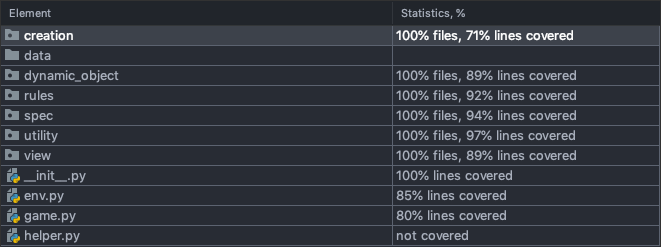
\includegraphics[scale=0.5]{images/coverage_script_manual.png}

	Le profilage de script\_manual.py montre la répartition du temps dans le code disponible dans images/profiling\_script\_manual.png. Une partie importante du temps est
	passé à attendre entre chaque itération de l'environement principal. Sinon, il n'y a pas de gros problème apparent.\\


	Pour conclure, l'ensemble des tests évitent d'avoir des bugs importants même si cela ne garantit pas que le code est parfait.
	Nous avons fait le plus de tests unitaire possible dans le temps imparti. Les tests permettent au projet d'être réutilisé
	et éviter que de futures modifications causent une régression.

	\newpage
	\section{Conclusion}
	Nous ne sommes pas forcément satisfait du code que nous avons rendu. Nous avons essayé de définir une architecture intéressante et d'avoir une bonne organisation du code. Mais nous avons fournit un travail un peu trop scolaire et l'architecture est trop complexe par rapport aux fonctionnalités que nous devions implémenter et qu'à coté il y a des fonctions statiques qui ne couvrent qu'un seul cas d'utilisation. Nous avons énormément de code dupliqué et de dépendances.\\

	Nous avons un gros problème de conception car on peut seulement lancer des matchs de la Robocup en 2vs2 alors que nous devions pouvoir au minimum lancer des matchs en 4vs4. Notre simulation est beaucoup trop statique. Nous avons utilisé le code de l'extension de slimvolleyGym pour aller plus vite sauf que nous nous sommes concentrés sur l'architecture et des fonctionnalités plus secondaire de notre simulation et finalement le contrat n'est pas rempli. Il suffisait juste d'adapter l'espace d'observation (voir besoin \ref{besoinObs}) de l'agent et le constructeur de \textbf{Team} (voir besoin \ref{besoinTeam})  pour pouvoir choisir la taille d'équipe que nous souhaitions, il fallait aussi faire une fonction pour placer les équipes sur le terrain en fonction de leur taille. \\
	Finalement en se basant sur des fonctions non adaptées au but d'origine on s'est retrouvé à adapter notre objectif à ces fonctions et on a perdu en pertinence, efficacité et utilité de l'application. On a plus une application qui fait office de jeu qu'une simulation paramétrable de la Robocup qui fournit différents environnements d'entrainement. \\
	Pour aller plus vite on a fait des concessions mais on se retrouve avec une un fonctionnement moins naturel : par exemple au lieu d'attribuer des numéros à nos agents on leur attribue des couleurs (nous avons rencontré des difficultés pour afficher des chiffres avec la fonction render de Gym). Avec 4 agents ce n'est pas un problème mais avec 8 c'est déjà ingérable.\\
	Pour tester nos environnement nous avons du adapter les scripts qui étaient obsolètes ce qui nous a fait perdre en efficacité. Nous avons réussi à faire un script d'entrainement mais c'est insuffisant pour prouver que l'on peut entrainer dans notre simulation.

	Il y a eu des problèmes de communication et de répartition du travail dans le groupe, si bien que toute une partie de code faite sur le CSV ou le JSON n'est pas ou très peu utilisée. On a aussi modifier l'architecture globale du code à une semaine et demi du rendu.\\
	Dès le début nous avons eu des problèmes de gestion du temps, nous avons compris le but du premier rapport seulement une semaine avant le rendu. Nous avons eu énormément de difficulté a entrer dans les détail à 6 sur un vocal discord et nous n'avons jamais pu nous poser et discuter des concepts calmement. Nous sommes déçus d'être passé à coté. \\

	Nous aurions aimé avoir ces points dans notre simulation :

	\begin{itemize}
		\item pouvoir choisir la taille d'une équipe dynamiquement
		\item différencier les agents avec des numéros plutôt que des couleurs
		\item rajouter des pénalités comme immobiliser un agent et donner la balle à l'adversaire en cas de faute.
		\item pouvoir modifier plus de paramètres
		\item faire des fonctions pour avoir des scripts généraux et que l'application soit plus simple d'utilisation
	\end{itemize}

	\section{Bibliographie}
	\bibliographystyle{elsarticle-num}
	\bibliography{Sources}

\end{document}
